% ============================================================
%  K. Kroman, »Relativitetsprincipet«
%  Fysisk Tidsskrift, 14. Aargang (1915-16), pp. 1-30.
%
%  DIPLOMATIC TRANSCRIPTION (Danish)
%  Status: COMPLETE. Printed pp. 1-30, all 30 pages, transcribed 2026-09-04
%  from the scan described below. No gaps, no duplicates; braces and guillemets
%  balanced; compiles with 0 errors, 0 missing characters, 0 overfull and 0
%  underfull boxes (26 LaTeX pages). English translation not begun.
%
%  Kroman's attack on special relativity, and the opening move of the only
%  sustained critical discussion the theory received in Denmark. The debate
%  runs to seven items; note.md in this directory carries the table, the
%  sourcing and Høffding's reply to it in Relation som Kategori (1921).
%
%  RIGHTS: clear. Kroman died 26 July 1925; Danish copyright (life+70) expired
%  at the end of 1995. Free to transcribe and to publish.
%
% ------------------------------------------------------------
%  THE WITNESS
% ------------------------------------------------------------
%  Google Books `Tr4ZAAAAIAAJ` -- Fysisk tidsskrift, VOLUMES 13-15 bound
%  together, the University of California copy, digitised 17 January 2007,
%  886 pages, full view. Kept as texts/kroman/scan-ft-13-15.pdf, untracked
%  (the root .gitignore excludes texts/**/scan*.pdf); the same file serves the
%  sibling articles in ../holst-tidsproblemet and ../yderligere-bemaerkninger.
%
%  The scan carries a usable Antiqua text layer -- accurate at the word level,
%  ae/oe/aa correct -- so it is the PRIMARY witness for the words, with
%  tesseract as second witness and the page image as arbiter for structure,
%  emphasis and mathematics. Every page of this article was inspected as an
%  image; the mathematics and every emphasis run were checked at 400-700 dpi.
%
%  KB catalogues only the offprint (30 s., »Særtryk af: Fysisk Tidsskrift XIV.
%  1. Hefte«), filed in the Særtrykssamlingen with no call number. That is why
%  two attempts to have KB produce this text failed. See note.md.
%
% ------------------------------------------------------------
%  PAGE MAP -- VERIFIED 2026-09-04
% ------------------------------------------------------------
%      printed 1-30  =  PDF + 330   (PDF 331-360), uniform.
%
%  Measured with `pagemap.py --detect` and then confirmed by reading the pages.
%  THE NUMERALS ALONE DO NOT IDENTIFY THIS ARTICLE: the file binds three
%  volumes and each has its own pp. 1-30, so offsets 12, 330 and 602 all fit
%  the running-head numerals perfectly. The tie was broken on content --
%      PDF 331 = printed 1   opens »Relativitetsprincipet«. / Af / K. Kroman.
%      PDF 345 = printed 15  carries »Sandheden er ikke dobbelt. Sandheden er
%                            kun én.«, the sentence Høffding cites in Relation
%                            som Kategori (1921) p. 75 n. as »XIV, p. 15«
%      PDF 361 = printed 31  is a different item (»Referat.«), so 30 is the end
%  Offset 602 turned out to be Holst's »Tidsproblemet« in vol. 15. Note that
%  the offset is NOT constant across the bind -- it is 622 by vol. 15 p. 192 --
%  because unpaginated advertisement leaves are bound in.
%
% ------------------------------------------------------------
%  CONVENTIONS -- SETTLED AGAINST THE IMAGES
% ------------------------------------------------------------
%  * Diplomatic. 1915 orthography exactly as printed: the pre-1948 aa kept,
%    nouns capitalised, nothing modernised.
%  * TYPEFACE: Antiqua, not Fraktur. The Fraktur OCR model and sed tables used
%    by the nineteenth-century books in this repo do not apply here.
%  * QUOTATION MARKS: GUILLEMETS »...«, set \guillemotleft / \guillemotright.
%    NOT the low-high pair „...“ of the nineteenth-century books. 15 pairs,
%    balanced. (The Google text layer renders them as ASCII > and <; ocr.sh
%    normalises them.)
%  * EM DASH ---.
%  * EMPHASIS is LETTERSPACING (Sperrsatz) throughout, set \emph{}. 146 runs.
%    Used for names, book titles and ordinary words alike. A possessive or
%    adjectival suffix normally falls OUTSIDE the spaced run -- \emph{Einstein}ske,
%    \emph{Newton}'sk -- but the printing is NOT consistent: \emph{Doppler'ske}
%    (p. 23), \emph{Michelson'ske} (p. 30) and \emph{Einsteins} (p. 29) carry
%    the suffix inside the run. All three verified at 600-700 dpi and set as
%    printed. One spaced run breaks across the p. 18/19 turn and is held
%    together with \-%.
%  * TRUE ITALIC occurs, and only for Latin tags: »Diversi respectus...«
%    (p. 15), »ratio sufficiens« (p. 18). Set \textit{}. No small caps anywhere.
%  * FOOTNOTES: the printing marks them *), at most one per page, on pp. 4, 6,
%    8, 16, 20, 28, 29. \thefootnote is fixed to *) in the preamble; the
%    counter still increments but is never shown. Footnote text is not always
%    letterspaced where the body would be (p. 16).
%  * MATHEMATICS. Variables italic, as the printing sets them. Built-up
%    fractions inline in the run of text use \dfrac, small ones \tfrac; case
%    fractions are written as printed. Greek (α β ε μ ν π λ) is set with
%    ordinary math commands; on p. 25 Greek ν and italic v stand side by side
%    in one formula and the distinction is load-bearing. »tg« for the tangent
%    is kept as printed (\mathit{tg}), not turned into \tan.
%  * EQUATION NUMBERS. The printing gives a flush-right BARE numeral with a
%    full stop and no parentheses, so \tag*{} is used, not \tag{}. Numbering
%    runs 1.-10. and then STOPS: the eighteen displays on pp. 21-30 are
%    unnumbered, and the text refers back to »Formlerne 9«, »ifølge 10«.
%  * The old Danish id-est sign ɔ: (p. 19) is built from a reflected c; see
%    the preamble.
%
% ------------------------------------------------------------
%  PRINTER'S DEFECTS -- transcribed AS PRINTED, logged at the site
% ------------------------------------------------------------
%    p.  4  »vinkelret paa den, Da Jordens« -- comma for a full stop
%    p. 10  »maaa« for »maa«
%    p. 13  h_z for h'_z -- a dropped prime in the marked velocities
%    p. 17  »B's'« -- a second apostrophe where the sense wants »B's«
%    p. 20  x_2' where the rest of the page sets x'_1 -- prime misplaced
%    p. 24  a full stop, not a colon, before the Fizeau display
%    p. 28  »for lidt*).« vs p. 29 »Brug for.*)« -- the footnote mark sits on
%           opposite sides of the stop
%    p. 30  »L o r e n t z-/ske Forkortning« -- no apostrophe and no spacing on
%           the suffix, where the rest of the page reads »L o r e n t z'ske«
%    p. 30  »Lorentz-Einstein-Transformationen« not letterspaced, though both
%           names are letterspaced everywhere else
%  Each is verified on the image at 600-700 dpi. None affects the guillemet
%  balance, which is 15/15 with zero drift.
%  NOT a defect of ours but worth recording: the RUNNING HEAD on p. 27 reads
%  »Relativitetprincipet« -- the s is dropped.
%
% ------------------------------------------------------------
%  THE FIGURE ON p. 5
% ------------------------------------------------------------
%  Printed p. 5 carries a line diagram of Michelson's apparatus, centred,
%  unnumbered and uncaptioned. It is REDRAWN IN TIKZ at the site -- an
%  editorial reconstruction, NOT a facsimile. Drawn 2026-09-04 from the scan
%  at 600 dpi, with the geometry measured off the image pixel by pixel
%  (O_1 and O_2 at +120 and +241 px from O; B 601 px above O; A at +596,
%  A_1 at +718), and set at 5.3 cm in a 14.9 cm measure -- the same 36 % of
%  the measure the original occupies.
%
%  Regularised, deliberately, and listed again in the comment above the
%  drawing itself:
%    * the mirror stroke at O is asymmetric in the printing; drawn symmetric
%    * the two mirror strokes at the top are drawn as one broken line
%    * the printing's dash runs vary from 12 to 28 px; drawn uniform
%  Not determined: whether the 45° diagonal at O is to scale, and where the
%  dashed continuation of the base line is meant to stop. Both are reproduced
%  as measured rather than as guessed.
%
%  A reader who needs the figure exactly as printed should go to the scan.
%
% ------------------------------------------------------------
%  BUILD
% ------------------------------------------------------------
%  pdflatex path (libertinus + libertinust1math), so the Makefile's default
%  pattern rule builds it. Sandbox compile-test per TRANSCRIPTION-PLAYBOOK.md §5.
% ============================================================

\documentclass[12pt,a4paper]{article}
\usepackage[utf8]{inputenc}
\usepackage[T1]{fontenc}
\usepackage{libertinus}
\usepackage{libertinust1math}
\usepackage{textalpha}   % Greek in text, typed directly
\usepackage{amsmath}     % this article has real formulas; see CONVENTIONS
\usepackage{graphicx}    % for \reflectbox, below
\usepackage{tikz}        % for the redrawn Michelson diagram, printed p. 5
% The old Danish id-est sign »ɔ:« (p. 19). T1 has no OPEN O, so it is built
% from a reflected c, as texts/brochner/det-religioese does.
\DeclareUnicodeCharacter{0254}{\reflectbox{c}}

% FOOTNOTES. The printing marks them *) and carries at most one per page
% (pp. 4, 6, 8, 16, 20, 28, 29), so a fixed mark is correct here; the counter
% still increments but is never shown.
\renewcommand{\thefootnote}{*)}
\usepackage[danish]{babel}
\usepackage[protrusion=true,expansion=true]{microtype}
\usepackage{setspace}
\usepackage[margin=1.2in]{geometry}
\usepackage{fancyhdr}
\setlength{\headheight}{15pt}
\usepackage{hyperref}

\hypersetup{
  pdftitle={Relativitetsprincipet},
  pdfauthor={K. Kroman},
  hidelinks
}

\pagestyle{fancy}
\fancyhf{}
\fancyhead[LE,RO]{\thepage}
\fancyhead[RE]{\textit{Relativitetsprincipet}}
\fancyhead[LO]{\textit{K. Kroman}}

\setstretch{1.3}

\title{\textbf{\guillemotleft Relativitetsprincipet\guillemotright}}
\author{K.\ Kroman}
\date{\textit{Fysisk Tidsskrift} 14 (1915--16), pp.~1--30}

\begin{document}
\maketitle

% --- p. 1 ---
\begin{center}
I.
\end{center}

Det er karakteristisk for den nyere Tid, at flere af de stringentere
Videnskaber har naaet en saadan Udviklingsgrad, at de vedkommende Forskere
har følt sig foranledigede til nøjere at undersøge Paalideligheden af selve
den Grundvold, paa hvilken deres Videnskab hviler. Saaledes har Matematikerne
allerede i en Aarrække syslet med Undersøgelser angaaende Geometriens
Fundament, et Arbejde, der som bekendt foreløbig har ført til det lidet
fornøjelige Resultat, at der end ikke paa matematisk Omraade længer er Enighed
blandt Menneskene, idet én Kreds af Forskere hævder, at det \emph{Euklidiske}
Grundlag vedblivende er det eneste rette, medens en anden Kreds finder det
rigtigere at opstille indtil en halv Snes forskellige ligeberettigede
Systemer, hvoraf \emph{Euklids} kun er ét.

Ogsaa paa Fysikkens Omraade har der i de senere Aar gjort sig
Relativitetsbestræbelser af forskellig Art gældende. \emph{Newton} var som
bekendt den, der først klart og udtømmende opstillede et alment Grundlag for
Fysikken --- som den kendtes paa hans Tid. Men den bestod den Gang væsenlig
alene af, hvad vi nu kalder den mekaniske Fysik. Af den nuværende Fysiks
øvrige Hovedafdelinger var der endnu kun svage Spor. Baade \emph{Huygens}' og
\emph{Newton}'s Optik var endnu væsenlig rent mekaniske. I vore Dage er der
navnlig kommet en omfattende Elektricitetslære til, og der er dermed bl.\ a.
opstaaet det Spørgsmaal: Kan ogsaa de mangfoldige elektriske Fænomener
forklares ud fra det \emph{Newton}'ske Grundlag, eller kræver dette nu
Tilføjelser, ja maaske endog Omformninger?
% The foot of p. 1 carries the signature line »Fysisk Tidsskrift. XIV.« with
% the sheet number »1« at the outer edge; p. 3 carries »1*«. Signature marks
% are not text of the work and are not transcribed.

% --- p. 2 ---
Paa Grund af den ufuldkomne Viden, vi endnu har om Elektricitetens egenlige
Natur, vil der dog sikkert gaa endnu en Tid, før der kan opstilles et
fuldtbegrundet Svar paa det nævnte omfattende Spørgsmaal, og det er da heller
ikke dette Problem, der skal omhandles paa de følgende Blade. Det er derimod
et Relativitetsproblem af en noget snævrere Art, nemlig den
\emph{Einstein}'ske Hypotese til Forklaring af det \emph{Michelson}'ske
Lyshastighedseksperiment, der skal gøres til Genstand for et Par kritiske
Bemærkninger.

A. \emph{Einstein} fremsatte først sine Anskuelser i \emph{Annalen der
Physik}, 1905, og hans Afhandling er tillige med flere andre om samme Emne
udgivet 1913 som et særligt lille Skrift med Titelen: H.\ A. \emph{Lorentz},
A. \emph{Einstein}, H. \emph{Minkowski}: \emph{Das Relativitätsprinzip}.

Den \emph{Einstein}'ske Hypotese, der fornemmelig bygger paa den
Forudsætning, at det er os umuligt at gøre Forskel paa Hvile og jævn retlinjet
Bevægelse, vakte straks en betydelig Opmærksomhed og fandt en ikke ringe
Tilslutning; der fremkom en ret frodig Litteratur, som behandlede Problemet og
søgte at gennemføre det videre. Der var dog ogsaa mange, der stillede sig ret
skeptisk overfor hans Tanker, og blandt andre har baade H. \emph{Poincaré} (i
et Foredrag holdt i Berlin: \emph{Die neue Mechanik}, udkommet i 2. Oplag
1913) og H. A. \emph{Lorentz} (i \emph{Das Relativitätsprinzip}, 3
Forelæsninger, 1914) særlig udtalt sig tvivlende om, hvorvidt den antydede
Udvej lader sig forlige med den menneskelige Erkendelses Grundbetingelser.
% A speck of dirt stands between »antydede« and »Udvej« in the scan; the
% pdftotext layer reads it as a full stop. There is no point on the image.

Det forekommer mig, at de nævnte betydelige Forskere har Ret i deres antydede
Tvivl, og det er da særlig den \emph{Einstein}'ske Hypotese set fra den
erkendelsesteoretiske Side, der i det følgende skal søges nærmere undersøgt.

\begin{center}
II.
\end{center}

Relativitetshypotesens første Foranledning var visse Lysfænomener. Lyslæren
synes i det hele at være et af Fysikernes Smertensbørn. \emph{Huygens}
opstiller sin Bølgeteori; men \emph{Newton} gør opmærksom paa, at
Bølgebevægelser kan bøje om Hjørner, medens Lysstraalerne tilsyneladende
aldrig gør dette. Heller ikke Polarisationen kunde Bølgeteorien klare, da man
foreløbig kun tænkte sig Længde\-%
% --- p. 3 ---
svingninger. \emph{Newton} opstiller derfor sin Emissionsteori, der vinder
almindelig Indgang og holder sig, indtil det viser sig, at ogsaa den fører til
Modsigelser. Vanskelighederne ved Bølgeteorien er imidlertid fjernede, bl.\ a.
idet man har ombyttet Længdesvingningerne med Tversvingninger. Uheldigvis maa
imidlertid Svingninger være Svingninger af noget eller i noget, og man førtes
derved til at opstille det mærkelige \guillemotleft Medium\guillemotright, som
man kalder Æteren. Det var Æterens Elasticitet, der skulde vedligeholde de
hurtige Svingninger. Man maatte derfor tilskrive den en utrolig stor
Elasticitetskoefficient; ja, da det var Tversvingninger, maatte man nærmest
opfatte den som en Art fast Legeme, mens man samtidig fandt, at den
tilsyneladende ikke ydede Verdenskloderne den allerringeste Modstand. Ad
matematisk Vej udformedes Teorien imidlertid finere og finere, saa at den
efterhaanden kunde give den ypperligste Løsning af en Mængde Enkeltproblemer,
og de mange elegante Resultater kastede til Dels et Slør over den skøre
Grundvold. Et væsenligt Fremskridt skete desuden ved, at \emph{Maxwell}
ombyttede de elastiske Svingninger med elektromagnetiske. Tversvingningerne
blev derved forklarlige, og Æteren mistede noget af sin Mærkværdighed. Men et
gaadefuldt Medium vedblev den dog ogsaa under de \emph{Maxwell}'ske
Forudsætninger at være, og ogsaa i sin sidste Form skulde Teorien snart føre
til tilsyneladende uovervindelige Vanskeligheder.

Det var lykkedes at finde Lysets Hastighed i Verdensrummet, i Luften, i Vand
og i en Mængde andre Legemer. Man mente endvidere at have fundet en ganske
simpel Forklaring paa det astronomiske Fænomen Aberrationen. Tænkes en Kikkert
fra Jorden pegende lige mod Solen, vil en Lysstraale, der netop træffer Midten
af Objektivet, ikke træffe Midten af Okularet; thi mens Lyset gennemløber
Kikkertens Længde, er Jord og Kikkert rykket $^{1}\!/_{10\,000}$ af denne
% Printed as a case fraction: raised 1, solidus, lowered 10 000 (thin space
% inside the numeral). Transcribed in that form, not as a built-up fraction.
Længde til Siden, saa at Straalen vil danne en Vinkel med Kikkertens Akse af
omtrent 20,5 Buesekunder. Saa naturlig og nærliggende denne Forklaring end
synes at være, rummer den dog en bestemt positiv Forudsætning, nemlig den, at
Lysstraalen beholder sin Retning i Rummet, mens Kikkerten rykker til Siden, og
at Æteren, hvori Lysbevægelsen foregaar, altsaa hviler i Rummet og ikke slæbes
med ved Jordens Bevægelse. Det er Hypotesen om \emph{den hvilende Æter}, der
dermed er opstillet. Den er, som man ser, i god Overensstem\-%
% --- p. 4 ---
melse med den Omstændighed, at Kloderne synes at kredse uden at lide ringeste
Modstand fra Æteren.

\emph{Airy} fyldte en Kikkert med Vand og fik gennem den dog den sædvanlige
Aberrationskonstant; dette Eksperiment kunde synes skæbnesvangert for den
sædvanlige Aberrationsteori, da Lyset bruger $^{4}\!/_{3}$ Gange saa lang Tid
i Vand som i Luft. Men det er jo muligt, ja sandsynligt, at Lyset ikke kan
bevæge sig gennem Vand, der har en Sidehast af 30 km i Sekundet, uden at faa
en Del af Vandets Hastighed med, og fik det f. Eks. $^{1}\!/_{4}$ af denne,
var jo alt i Orden. Nu har baade \emph{Fizeau} og \emph{Michelson} ved Forsøg
paavist, at Lyset ved at gaa gennem Vand med Hastighed i Lysstraalens Retning,
faar en Del af Vandets Hastighed i Tilgift. \emph{Fresnel} havde ud fra visse
Forudsætninger om Æteren forudsagt, at denne Tilgift maatte blive
$\dfrac{n^{2}-1}{n^{2}}$ Gange Vandets Hastighed, idet $n$ er Vandets
% Set as a built-up fraction standing in the run of the line, not displayed.
Brydningskoefficient. Ud fra nyere Forudsætninger er man kommet til samme
Resultat, og de to Forskeres Forsøg bekræftede fuldstændig dette.

Den afgørende Vanskelighed for den gængse Fysik indtræder derfor først med
A. \emph{Michelson}'s berømte Eksperiment. Dette er allerede tidligere
udførlig beskrevet her i Tidsskriftet\footnote{10. Aargang, Side 257.}. Det
vil derfor være tilstrækkeligt kort at erindre om dets Hovedpunkter.

\begin{center}
III.
\end{center}

\emph{Michelson}, der var berømt for sine fine Interferensforsøg, ventede
sikkert ved et saadant at kunne levere et Stuebevis for Jordens Translation,
ligesom \emph{Foucault} ved sit Pendul og sit Gyroskop havde leveret et
Stuebevis for dens Rotation. Han vilde med andre Ord prøve, om man ikke ved
Hjælp af Interferensstribernes Forskydning kunde spore Forskel paa den Tid,
Lyset var om at løbe en vis relativ Strækning frem og tilbage, naar Vejen den
ene Gang faldt i Jordens Translationsretning og den anden Gang stod vinkelret
paa den, Da Jordens Translationshastighed er omtrent 30 km i Sekundet, altsaa
% PRINTER'S ERROR, p. 4: »vinkelret paa den, Da Jordens« -- a comma where the
% sense and the following capital D require a full stop. Transcribed as
% printed. Verified on the image at 260 dpi.
omtrent en Titusindedel af Lysets Hastighed i Verdensrummet og Luften, syntes
dette ham ikke umuligt. Han udsendte
% --- p. 5 ---
da parallelle Lysstraaler fra $L$, som ved Hjælp af et svagt belagt Planspejl
i $O$ delte sig, saa at nogle gik den ene, andre den anden af de to Veje frem
og tilbage, hvorpaa de atter forenede sig i $O$ og gik til Kikkerten i $K$.
Var de relative Veje lige lange, maatte de mere absolutte jo blive
forskellige, og de genforenede Straaler maatte da vise Forskydning af
Interferensstriberne. Hele hans Apparat svømmede paa Kviksølv og kunde uden at
komme i mærkbar Uorden drejes, saa at snart det ene og snart det andet Sæt
Straaler gik den længste af de to Veje.

% ================================================================
% FIGURE, printed p. 5.  EDITORIAL REDRAWING IN TikZ -- NOT A FACSIMILE.
% Drawn 2026-09-04 from the page image at 600 dpi (PDF 335), by measuring
% the printed strokes pixel by pixel and then regularising them; no part
% of the original block is reproduced photographically.
%
% MEASURED FROM THE SCAN (600 dpi pixels, origin at O, y upwards):
%   O = 0, O_1 = +120, O_2 = +241, A = +596, A_1 = +718 on the base line;
%   B and B_1 stand 601 above O and O_1.  Base line solid from x = -124
%   to A, dashed on to +839; vertical at O from B down to -110 (towards K).
%   The two spacings O--O_1 and O_1--O_2 measured 120 and 121 px, i.e.
%   equal, and are set equal here.
%
% WHAT IS DRAWN, and how it differs from the printing:
%   * The apparatus is at full stroke weight, the ray path OB_1O_2 at
%     about half -- a distinction the printing makes and that is kept.
%   * The displaced positions (mirror at B_1, the vertical at A_1, and
%     the base line beyond A) are DASHED in the printing at full weight;
%     so here.  The ray path is a finer dotted line; so here.
%   * The half-silvered mirror at O measured 74 px up-right of O and 62 px
%     down-left, at 45 degrees.  REGULARISED to a symmetric +-70 px stroke:
%     the asymmetry is within the tolerance of a hand-drawn block.
%   * The solid mirror stroke at B measured 93 px left of B and 74 right,
%     the dashed one at B_1 38 left and 77 right.  REGULARISED: the two
%     strokes are drawn as one broken line, solid to midway between B and
%     B_1 and dashed thence to the end, which is what the block looks like.
%   * Dash lengths in the printing are irregular (on-runs of 12-28 px);
%     REGULARISED to a uniform pattern.
%   * COULD NOT BE DETERMINED: whether the short diagonal at O is meant to
%     be drawn to scale as a mirror of definite size, and whether the
%     dashed base line beyond A_1 is meant to stop where it does or is
%     simply where the engraver ran out; both are reproduced as measured.
%   * The block is 4.3 cm wide on the printed page against a 11.9 cm text
%     block, i.e. 36 percent of the measure; drawn here at 5.3 cm against
%     14.9 cm, i.e. the same proportion of this edition's measure.
%
% All letters are italic in the printing and are set as math italic here;
% the subscripts are 1 and 2.  Positions of the letters follow the block.
% ================================================================
\begin{center}
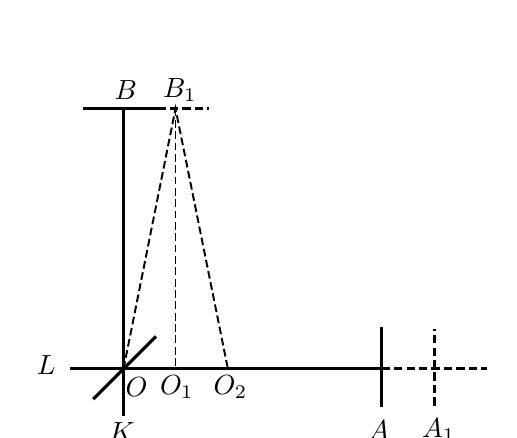
\begin{tikzpicture}[x=0.55cm,y=0.55cm,
    apparatus/.style={line width=1.2pt},
    ray/.style={line width=0.7pt,dash pattern=on 2.8pt off 1.3pt},
    broken/.style={line width=1.2pt,dash pattern=on 3pt off 1.5pt}]

  % --- the base line: Jordens Translationsretning ---
  \draw[apparatus] (-1.24,0) -- (5.96,0);          % L ... O ... A, solid
  \draw[broken]    (5.96,0) -- (8.39,0);           % beyond A, dashed

  % --- the vertical arm, O up to B and down towards the telescope K ---
  \draw[apparatus] (0,-1.10) -- (0,6.01);

  % --- the end mirror at B, and its displaced position at B_1 ---
  \draw[apparatus] (-0.93,6.01) -- (0.78,6.01);
  \draw[broken]    (0.78,6.01) -- (1.97,6.01);

  % --- the lightly silvered plane mirror at O, at 45 degrees ---
  \draw[apparatus] (-0.70,-0.70) -- (0.75,0.75);

  % --- the end mirror at A, and its displaced position at A_1 ---
  \draw[apparatus] (5.96,-0.87) -- (5.96,0.96);
  \draw[broken]    (7.18,-0.85) -- (7.18,0.91);

  % --- the ray's actual path O B_1 O_2, and the perpendicular B_1 O_1 ---
  \draw[ray] (0,0) -- (1.20,6.01) -- (2.41,0);
  \draw[ray] (1.20,6.01) -- (1.20,0);

  % --- lettering ---
  \node[anchor=east]  at (-1.34,0.08) {$L$};
  \node               at ( 0.30,-0.42) {$O$};
  \node               at ( 1.23,-0.42) {$O_{1}$};
  \node               at ( 2.47,-0.42) {$O_{2}$};
  \node               at (-0.04,-1.47) {$K$};
  \node               at ( 0.05, 6.44) {$B$};
  \node               at ( 1.30, 6.44) {$B_{1}$};
  \node               at ( 5.90,-1.42) {$A$};
  \node               at ( 7.28,-1.42) {$A_{1}$};
\end{tikzpicture}
\end{center}

Har Jordens Bevægelse Retning $OA$, og er $OA = OB = l$, vilde en Lysstraale
--- mente han ---, hvis Jorden stod stille, bruge Tiden $\dfrac{2l}{c}$ til at
gaa frem og tilbage mellem $O$ og $A$ eller $B$, idet $c$ er Lysets Hastighed.
Men har Jorden selv Hastigheden $v = \dfrac{c}{10\,000}$, maa den Straale, der
gaar til $A$ (som samtidig kommer til $A_{1}$) til Henvejen bruge Tiden
$t_{1} = \dfrac{l+vt_{1}}{c} = \dfrac{l}{c-v}$ og til Tilbagevejen Tiden
$t_{2} = \dfrac{l-vt_{2}}{c} = \dfrac{l}{c+v}$, altsaa ialt Tiden
$t = \dfrac{2l}{c}\cdot\dfrac{1}{1-v^{2}/c^{2}}$.
% »ialt« here, »i alt« three lines below and again on p. 10. As printed.

Den Straale, der gaar til $B$, vil paa Grund af Jordens Bevægelse gennemløbe
Vejen $OB_{1}O_{2}$ og maa derfor til Henvejen bruge Tiden
$t_{3} = \dfrac{\sqrt{l^{2}+v^{2}t_{3}^{2}}}{c}$ og til Hjemvejen samme Tid,
altsaa i alt Tiden $t' = \dfrac{2l}{c}\dfrac{1}{\sqrt{1-v^{2}/c^{2}}}$.

% --- p. 6 ---
Vejforskellen for de to Straaler bliver saaledes med stor Tilnærmelse
\[
  F = 2l\left[\frac{1}{1-v^{2}/c^{2}} - \frac{1}{\sqrt{1-v^{2}/c^{2}}}\right]
    = 2l\left[1+\frac{v^{2}}{c^{2}}
      - \left(1+\frac{v^{2}}{2c^{2}}\right)\right]
    = l\frac{v^{2}}{c^{2}} = l\cdot 10^{-8}.
\]
% Displayed, centred, unnumbered; set as one line across the measure.

Ved \emph{Michelson}'s første Forsøg var\footnote{Ifølge \emph{Wüllner}:
\emph{Experimentalphysik}, 5. Aufl. IV, 607. Talstørrelserne angives i de
forskellige Beretninger yderst forskelligt. De spiller imidlertid i
nærværende Sammenhæng ingen væsenlig Rolle.} $l = 120$ cm, og det Lys, han
benyttede, havde Bølgelængden $\lambda = 60\cdot 10^{-6}$ cm. I et senere
Forsøg, han udførte sammen med \emph{Morley}, var $l$ ved Hjælp af Spejle
bleven forøget til 1200 cm. I første Tilfælde faas
$F = \dfrac{12\cdot 10^{-7}}{60\cdot 10^{-6}}\lambda = 0{,}02\lambda$, i sidste
$F = \dfrac{12\cdot 10^{-6}}{60\cdot 10^{-6}}\lambda = 0{,}2\lambda$. Man
maatte da vente en Forskydning af Interferensstriberne af henholdsvis 0,02 og
0,2 Stribebredders Størrelse, snart til den ene og snart til den anden Side,
efter hvorledes Apparatet orienteredes. Selv den mindste af disse
Forskydninger vilde ifølge \emph{Michelson} have været til at iagttage i den
med Okularmikrometer forsynede Kikkert, der benyttedes. Men end ikke i sidste
Tilfælde saas med Sikkerhed nogen Forandring i Stribernes Stilling.

Dette negative Resultat var unægtelig en Overraskelse, en Gaade, der bragte
Modsigelse ind i vor fysiske Viden. Det blev da Opgaven atter at faa fjernet
denne Modsigelse.

Den mest nærliggende Udvej blev baade forsøgt og spærret af \emph{Michelson}
selv. Han tænkte sig Muligheden af, at Jorden i Forsøgsøjeblikket heller ikke
havde nogen virkelig Translation, idet hele Solsystemet samtidig gik i modsat
Retning med 30 km's Hastighed. Han gentog derfor Forsøget, efter at
Translationsretningen var bleven en væsenlig anden. Men Resultatet forblev som
før.

Den næst nærmeste Udvej vilde være den at erklære Eksperimentet for
utilstrækkelig fuldkomment. Hvor det kun drejer sig om en Vejforskel af
Brøkdelen af en Lysbølgelængde, kan aabenbart selv de mindste Unøjagtigheder
ødelægge det hele. Selv den allerringeste Temperaturdifferens kunde jo
forandre Spejlenes indbyrdes Afstand tilstrækkeligt. Herpaa kan der imidlertid
svares, at Interferensstribernes Tydelighed og Forbliven paa Plads afgørende
viste,
% --- p. 7 ---
at Apparatet i øvrigt var i Orden og at det udtrykkelig var Vejforskellen, det
nægtede at vise Tegn paa.

Vi maa altsaa søge nye Udveje, og det metodisk rette er vel da, at vi først og
fremmest vender os mod selve den gængse Lysteori og spørger: Er den da
fuldstændig i Orden? Var det med Rette, man ventede de omtalte
Stribeforskydninger?

Her forekommer det mig, at der ligger et vidtudstrakt Felt for nærmere
Undersøgelser, et Felt, som sikkert ikke allerede kan være saa gennempløjet,
at man kan opgive al Søgen her og vende sig til allehaande fjernere liggende
mulige Udveje. Saa længe man har kendt Interferensfænomener, har de jo voldt
Forskningen Overraskelser, som det først efterhaanden lykkedes at magte. Véd
vi med tilstrækkelig Klarhed, hvorledes de lysende Legemer bærer sig ad med at
frembringe og udsende de mærkelige Lyssvingninger? Det er vel den almindelige
Opfattelse, at Lyset i Verdensrummet og i Atmosfæren bestandig udsendes og
forplanter sig med den konstante Hast $c = 300\,000$ km i Sekundet uafhængigt
af Lyskildens Hvile eller Bevægelse. Men hvor sikre Grunde har denne
Antagelse? Kunde det ikke tænkes, at den ret uvilkaarlig har dannet sig, blot
fordi de mulige Tilgifter eller Fradrag, der her kunde blive Tale om, forekom
saa betydningsløse? Man har villet forklare \emph{Michelson}'s Resultat ved
den Antagelse, at Lyset bestandig fik Lyskildens Hastighed med som Tilgift.
Der er rejst Indvendinger mod en saadan Opfattelse; men ogsaa mod disse
Indvendinger er der rejst Indvendinger. En lempeligere Antagelse var
imidlertid den, at Lyset i de første Øjeblikke fik Lyskildens Bevægelse med,
men hurtig gik over til den sædvanlige Hastighed. At den gængse Teori skulde
være saa fast udformet, at der slet ikke var Plads for den ene eller den anden
af saadanne Ændringer, er dog sikkert en forhastet Tro. Heller ikke Æterens
Forhold er vel endnu saa fastslaaet, at der ikke her skulde være Plads for en
eller anden Nuancering, der muliggjorde en Løsning af Gaaden. Adskillige
Eksperimenter er jo fulgt efter \emph{Michelson}'s med nærmest tilsvarende
negative Resultater. Men de væsenligste af dem har dog alle ligget paa
Lysfænomenernes Omraade, og det synes derfor ret rimeligt, at det ogsaa bør
være der, man først og fremmest spejder efter den forløsende Udvej.

Det ser imidlertid ud, som om Fysikerne allerede var bleven trætte af at søge
her. Det første Løsningsforsøg, der vandt en større
% --- p. 8 ---
Tilslutning, havde en langt bredere Basis. Det hidrørte fra H. A.
\emph{Lorentz} og udmærkede sig i ethvert Tilfælde ved, at det dog var et
virkelig \emph{fysisk} Løsningsforsøg.

\emph{Lorentz} mente, at det vilde støde paa uovervindelige Vanskeligheder at
tænke sig Æteren ført med af Legemerne, og han følte sig ligeledes overbevist
om, at Lyset bestandig har Hastigheden $c$ gennem Æteren og i Luften. Han
antog derfor, at \emph{Michelson}'s negative Resultat maatte bero paa, at
ethvert translatorisk bevæget Legeme lider en Sammentrækning i Bevægelsens
Retning netop saa stor, at bl.\ a. \emph{Michelson}'s Resultat derved bliver
forklarligt\footnote{Samme Udvej blev omtrent samtidig foreslaaet af
\emph{Fitzgerald}.}. Er Translationshastigheden $v$, bliver Legemets
Udstrækning i Translationsretningen ifølge Hypotesen
\[
  a = \frac{1}{\sqrt{1-v^{2}/c^{2}}}
\]
Gange saa lille, som den var under Hvile. Under \emph{Michelson}'s Forsøg
havde hans Apparat jo Jordens Translationshastighed, $v$. Det er altsaa i
denne Retning blevet $a$ Gange saa lille. Men netop derved er de to Lysveje
bestandig bleven lige lange.

\emph{Lorentz} bemærker, at denne Hypotese vel i første Øjeblik maa vække lidt
Undren. Men ved nærmere Betragtning bliver den dog ret naturlig og
nærliggende. Molekularkræfterne maa jo sikkert til syvende og sidst være
betingede af Æteren, og det kan da ikke overraske, at de ved Translationen kan
lide den antagne ringe Forandring. Thi det er kun en overordenlig ringe
Forandring, det drejer sig om. Størrelsen $a$ er kun ganske umærkeligt
forskellig fra 1. Jordens Banehast er omtrent 1800 Gange saa stor som et af
vore Iltogs, og Jordens Diameter er omtrent 12\,800 km. Og dog vilde dens
Forkortning kun beløbe sig til 6,4 cm. At ingen hidtil har lagt Mærke til, at
Tingene led en saadan Forkortning, kan altsaa ikke undre.

Dette er den \emph{Lorentz}'ske Forklaring af \emph{Michelson}'s negative
Resultater. Den udmærker sig som sagt ved at være en virkelig fysisk Hypotese,
der paa sin Maade virkelig forklarer, hvad der skulde forklares. Flere ---
saaledes blandt andre H. \emph{Poincaré} --- har imidlertid fundet det yderst
vanskeligt at antage en saadan fysisk Forkortning, der skulde være ens for de
forskelligste Legemer, blot
% --- p. 9 ---
disse havde samme Hastighed, og, som vi skal se, gaar den \emph{Einstein}'ske
Tankegang da ogsaa ud paa at forklare de vedkommende Resultater uden
Indførelse af nogen virkelig fysisk Forkortning, ja efter Einsteins egen
Opfattelse uden overhovedet at indføre nogen egenlig ny Hypotese.
% »efter Einsteins egen Opfattelse« is NOT letterspaced here, though every
% other occurrence of the name on pp. 1--10 is. Checked on the image.

\begin{center}
IV.
\end{center}

Den første Impuls til sit ejendommelige Løsningsforsøg har \emph{Einstein}
sikkert faaet fra den \emph{Lorentz}'ske Forkortningshypotese; men i øvrigt er
han gaaet sine ganske særlige Veje. Vi vil begynde med at udlede hans berømte
Formler uden endnu at bygge paa hans særlige Forudsætninger. Disse Formler kan
nemlig faas ud fra flere forskellige Udgangspunkter og tilmed ad ganske
elementær Vej, og gaar vi saaledes frem, mens vi foreløbig holder os til
ganske almindelige Forudsætninger, vil vi dels muligt opnaa at faa fjernet det
halvt mystiske Skær, som Formlerne ofte nok har faaet over sig, og dels vil
den paafølgende Overgang til de særlige \emph{Einstein}'ske Forudsætninger
tydeligst lade disse fremtræde i deres fulde Ejendommelighed. Vi vil trods
dette ikke behøve at fjerne os ret langt fra hans egen Fremstilling.

Vi tænker os da i Rummet to retvinklede Koordinatsystemer, $Oxyz$ og
$O'x'y'z'$. I et vist Øjeblik falder de fuldstændig sammen; men det sidste har
i Forhold til det første en Translation i X-aksens Retning med den konstante
% X here is upright roman in the printing; on p. 10 the same axis is set
% italic as X'. Both readings kept as printed.
Hastighed $v$. Vi kan tænke os en legemlig Verden knyttet til ethvert af de to
Systemer og antage en Iagttager, A, i det første og en Iagttager, B, i det
andet, hver med sine Medarbejdere forsynede med mekanisk fuldkomne Ure og
Maalestokke. Enhver af dem tror sit eget System hvilende og den andens
bevæget, og de antager begge, at Lyset i Verdensrummet og Luften har den
konstante Hastighed $c$ uafhængigt af Lyskildens Hvile eller Bevægelse. Det
gælder nu om at udfinde, hvad de i Henhold til deres forskellige
Forudsætninger maa mene om hinanden.
% The observers A and B are set in upright roman throughout pp. 9--10;
% the geometrical points of the p. 5 figure are italic. As printed.

Vi kan begynde med A. Han opstiller sine Ure paa forskellige Steder i sit
System og skaffer dem ens Gang og Stand ved at udsende Lyssignaler, der kastes
tilbage til Udgangspunktet. Lad begge Systemers Begyndelsespunkter regne Tiden
fra deres Sammentræfsøjeblik, og lad os for Nemheds Skyld antage, at alle
Operationer tager
% --- p. 10 ---
deres Begyndelse ved dette Tidspunkt. A sender altsaa ved Tiden 0 et Lyssignal
fra $O$ til Stedet $L$ i Afstand $l$. Ved Signalets Ankomst til $L$ skal Uret
der altsaa ifølge hans Forudsætning stilles paa $t_{1} = l/c$, og ved
Signalets Tilbagekomst til $O$ skal Uret der vise $t_{2} = 2l/c$. Paa denne
Maade søger A at skaffe alle sine opstillede Ure ens Gang og Visning.

B, der tror \emph{sit} System hvilende, bærer sig ad ganske paa samme Maade.
Han sender f. Eks. ved Tiden $t' = 0$ fra $O'$ et Signal langs $Y'$-aksen til
et Ur i Afstand $l$. Dette stilles ved Signalets Ankomst paa $t'_{1} = l/c$,
og Uret i $O'$ stilles ved Signalets Tilbagekomst paa $t'_{2} = 2\,l/c$.

Denne Fremgangsmaade staar imidlertid for A, der tror B's System bevæget, som
ganske urigtig. Han finder, at Lyset til Henvejen maa have brugt Tiden
$t_{1} = \dfrac{\sqrt{l^{2}+v^{2}t_{1}^{2}}}{c}$ og til Tilbagevejen samme
Tid, altsaa i alt Tiden
$t = \dfrac{2l}{c}\dfrac{1}{\sqrt{1-v^{2}/c^{2}}}$. Men sættes Størrelsen
\begin{equation}\tag*{1.}
  \frac{1}{\sqrt{1-v^{2}/c^{2}}} = a,
\end{equation}
% The only numbered equation on pp. 1--10. The number is printed as a bare
% arabic numeral with a full stop, »1.«, flush right on the line of the
% display -- not in parentheses. Kept with \tag.
finder A altsaa, at B's Tidsangivelser for saa vidt maaa blive $a$ Gange for
% PRINTER'S ERROR, p. 10: »maaa« for »maa«. Transcribed as printed;
% verified on the image at 800 dpi.
smaa og hans Tidsenheder (Sekunder) $a$ Gange for store. Og for B's
Lyssignaler langs $Z'$-aksen kommer han til samme Resultat.

Langs $X'$-aksen bliver Sagen imidlertid mere sammensat. B bærer sig her ad
som før. Men A finder, at sender B et Signal fra $O'$ til et Sted paa
$X'$-aksen i Afstand $l$, maa det til Henvejen bruge Tiden
$t_{1} = \dfrac{l+vt_{1}}{c} = \dfrac{l}{c-v}$ og til Hjemvejen Tiden
$t_{2} = \dfrac{l-vt_{2}}{c} = \dfrac{l}{c+v}$, altsaa i alt Tiden
$t = \dfrac{2l}{c}\dfrac{1}{1-v^{2}/c^{2}} = \dfrac{2l}{c}\cdot a^{2}$ og
altsaa $a$ Gange saa lang Tid som under de tilsvarende Forhold langs de andre
Akser.

Fandt en saadan Modsigelse virkelig Sted, maatte B imidlertid --- mener A ---
hurtigt have opdaget den. Thi det vilde jo da have været ham umuligt at faa
ordnet sit Ur i $O'$. Den kan derfor \emph{ikke} finde Sted. Men dette kan kun
tænkes muligt, saafremt alle $X'$-afstande $l$ i Virkeligheden kun har haft
Længden $l/a$. B's System maa altsaa paa Grund af sin Bevægelse have trukket
sig sammen, saa at det selv og alle Maalestokke og andre Legemer i det, der
har deltaget i Be\-%
% BATCH SEAM: printed p. 10 ends mid-word. »Be-« continues as »vægelsen« at
% the head of p. 11. The trailing % above eats the newline; run joins.py
% after splicing, and make sure no blank line lands between the two halves.
% --- p. 11 ---
vægelsen, er bleven $a$ Gange saa korte i $X'$-retningen, som de var
under Hvile. Er ogsaa Maalestokkene forkortede, forstaar man, at B intet
har mærket og at han vedblivende har maalt $X'$-længderne $\dfrac{l}{a}$
som $l$. Men antager man denne Forkortning, vil B's samtlige Signaler frem
og tilbage altsaa kun have brugt $a$ Gange saa lang Tid som af B beregnet,
og man faar da overalt i B's System (i Systemet hvilende) Ure, der gaar $a$
Gange for langsomt i Forhold til A's, altsaa for saa vidt en almindelig
A-tid og en almindelig B-tid.
% »Men antager man...« is NOT indented in the printing, but the line above
% it is justified to the right margin: it is the same paragraph running on,
% not a new one with a dropped indent. Set continuous here.

Dette gælder imidlertid kun Urenes Gang.

Thi med Hensyn til deres Stand er der for A endnu noget i Vejen. A fandt,
at Signalet i $X'$-retning til Henvejen maatte bruge A-tiden
$\dfrac{l}{c-v}$. Paa Grund af Forkortelsen maa dette rettes til A-tiden
$\dfrac{l}{a(c-v)}$, altsaa til B-tiden $\dfrac{l}{a^{2}(c-v)}$. Men B lod
Uret i hans Afstand $l$ stille paa Tallet $\dfrac{l}{c}$. Uret i
B-afstanden $l$ fra $O'$ i $X'$-retning er altsaa stillet, saa at det
ifølge A faar et Klokkesletsunderskud i B-tid af
% The superscript sort in this journal is a curled glyph that reads like a
% 3 at low resolution; it is a 2 throughout. Verified arithmetically here
% (1/a^2 = (c^2-v^2)/c^2 makes the chain come out) and at 600 dpi.
\begin{equation}\tag*{2.}
  u = \frac{l}{a^{2}(c-v)} - \frac{l}{c}
    = \frac{l(c^{2}-v^{2})}{c^{2}(c-v)} - \frac{lc}{c^{2}}
    = \frac{v}{c^{2}}\,l.
\end{equation}
% \tag* (not \tag) because amsmath's \tag would set the number in
% parentheses, and the printing gives a bare numeral with a full stop,
% flush right. The \tag{1.} on p. 10 needs the star too -- see the report.

A har saaledes endvidere fundet, at B's Ure har et Visningsunderskud
proportionalt med deres $X'$-afstande fra $O'$. Er denne Afstand negativ,
er Underskuddet negativt. I $O'$ er det 0. I System B er der for A altsaa
ikke blot B-tid, men tillige \emph{Stedtid}, omtrent ligesom vi her paa
Jorden ikke blot har Middeltid og Stjernetid, men endvidere Greenwichtid
og Stedtid eller Zonetid.

Lad der nu indtræde et eller andet momentant og punktuelt Fænomen, $F$,
som af A maa henføres til Tiden $t$ og Stedet $x$, $y$, $z$ og af B til
Tiden $t'$ og Stedet $x'$, $y'$, $z'$, og lad os bestemme Forholdene mellem
de 8 nævnte Størrelser.

Ifølge det foregaaende kan vi straks sætte
\begin{equation}\tag*{3.\quad 4.}
  y = y' \qquad\qquad z = z'
\end{equation}
% Two equations on one line share one flush-right tag, printed »3. 4.«.
Endvidere ses det let, at vi maa sætte
\begin{equation}\tag*{5.}
  t = a\left(t' + \frac{v}{c^{2}}\,x'\right).
\end{equation}

% --- p. 12 ---
Thi er $t'$ B-tiden paa Stedet $x'$, $y'$, $z'$, giver Parentesen os
B-tiden i $O'$, og A-tiden er netop $a$ Gange saa stor som denne.

For at faa Forholdet mellem $x$ og $x'$ sætter vi A's Koordinat
$x = m + n$, hvor $m$ er Afstanden fra $O$ til $O'$ ved A-tiden $t$, altsaa
$= vt$ eller ifølge 5 $= va\left(t' + \dfrac{v}{c^{2}}\,x'\right)$, medens
$n$ er $X'$-afstanden fra $O'$ til Fænomenet, altsaa $x'$ B-metre eller
$\dfrac{x'}{a}$ A-metre. Vi faar saaledes, idet
$\dfrac{1}{a^{2}} = \dfrac{c^{2}-v^{2}}{c^{2}}$,
% The 1/a^2 equality is a built-up fraction standing in the run of the
% sentence; it opens a line only because »Vi faar saaledes, idet« fills the
% line above. Not a display in the printing.
\begin{equation}\tag*{6.}
  x = a\left(x'\,\frac{v^{2}+c^{2}-v^{2}}{c^{2}} + vt'\right)
    = a\,(x' + vt').
\end{equation}

Af 5 og 6 faas $t'$, idet man har
\[
  t' = \frac{t}{a} - \frac{v}{c^{2}}\,x'
     = \frac{t}{a} - \frac{v}{c^{2}}\left(\frac{x}{a} - vt'\right);\quad
  t'\,\frac{c^{2}-v^{2}}{c^{2}}
     = \frac{1}{a}\left(t - \frac{v}{c^{2}}\,x\right)
\]
altsaa
\begin{equation}\tag*{7.}
  t' = a\left(t - \frac{v}{c^{2}}\,x\right).
\end{equation}

Og af 6 og 7 faas $x'$, idet
\[
  x' = \frac{x}{a} - vt'
     = \frac{x}{a} - avt + a\,\frac{v^{2}}{c^{2}}\,x
     = a\left(x\,\frac{c^{2}-v^{2}+v^{2}}{c^{2}} - vt\right);
\]
\begin{equation}\tag*{8.}
  x' = a\,(x - vt).
\end{equation}

I alt faas saaledes
\begin{equation}\tag*{9.}
  \left.
  \begin{array}{l@{\qquad\qquad}l}
    t = a\left(t' + \dfrac{v}{c^{2}}\,x'\right)
      & t' = a\left(t - \dfrac{v}{c^{2}}\,x\right)\\[3ex]
    x = a\,(x' + vt') & x' = a\,(x - vt)\\[1.5ex]
    y = y' & y' = y\\[1.5ex]
    z = z' & z' = z
  \end{array}
  \right\}
\end{equation}
% Two columns closed by one tall right brace, with the number beside it.

Som det ses, faas det ene Sæt Formler af det andet, blot vi lader $v$
skifte Tegn og forandrer de ikke mærkede Bogstaver til mærkede og omvendt.
Dette er et Udtryk for, at B maa mene akkurat det
% --- p. 13 ---
samme om A, som A mener om B, paa Hastighedsretningen nær, og dette kunde
vi have forudsagt, da B jo troede netop det samme om A som A om B med den
nævnte Forskel.

Af disse Grundformler kan naturligvis udledes en Mængde andre. Vi vil her
blot endnu tilføje Formlerne for den konstante Hastighed langs enhver af
Koordinatakserne. Begynder Bevægelsen i $O$ ved Tiden 0, har man jo
$h_{x} = \dfrac{x}{t}$, $h_{y} = \dfrac{y}{t}$, $h_{z} = \dfrac{z}{t}$ og
naturligvis $h'_{x} = \dfrac{x'}{t'}$, $h'_{y} = \dfrac{y'}{t'}$,
$h_{z} = \dfrac{z'}{t'}$. Men da faas af 9
% PRINTER'S ERROR, p. 13: the third of the mærkede velocities is set
% »h_z«, without the prime; the sense and the two members before it require
% h'_z. Transcribed as printed. Verified on the image at 600 dpi.
\[
  h_{x} = \frac{a(x' + vt')}{a\left(t' + \dfrac{v}{c^{2}}\,x'\right)}
        = \frac{h'_{x} + v}{1 + \dfrac{v}{c^{2}}\,h'_{x}}
\]
og ad samme Vej i det hele
\begin{equation}\tag*{10.}
  \left.
  \begin{array}{l@{\qquad\qquad}l}
    h_{x} = \dfrac{h'_{x} + v}{1 + \dfrac{v}{c^{2}}\,h'_{x}}
      & h'_{x} = \dfrac{h_{x} - v}{1 - \dfrac{v}{c^{2}}\,h_{x}}\\[5ex]
    h_{y} = \dfrac{h'_{y}}{a\left(1 + \dfrac{v}{c^{2}}\,h'_{x}\right)}
      & h'_{y} = \dfrac{h_{y}}{a\left(1 - \dfrac{v}{c^{2}}\,h_{x}\right)}\\[5ex]
    h_{z} = \dfrac{h'_{z}}{a\left(1 + \dfrac{v}{c^{2}}\,h'_{x}\right)}
      & h'_{z} = \dfrac{h_{z}}{a\left(1 - \dfrac{v}{c^{2}}\,h_{x}\right)}
  \end{array}
  \right\}
\end{equation}

Ved en let Differentiation faas de samme Udtryk for variable Hastigheder.
Samtlige Formler danner, hvad Matematikerne kalder \guillemotleft en
invariant Transformation\guillemotright.

\begin{center}
V.
\end{center}

Alt dette er imidlertid foreløbig blot en matematisk Fantasi. Vi skal nu
prøve at bringe den i Forhold til Virkeligheden. Først betragter vi den
paa ganske sædvanlig Maade.

A tror, hans System hviler. Lad os for at faa et bestemt Udgangspunkt
\emph{foreløbig} forudsætte, at han har Ret; ingen har jo tænkt paa rent
at afskaffe Begrebet Hvile. Endvidere nærer
% --- p. 14 ---
baade A og B den sædvanlige Opfattelse, at Lyset uafhængigt af Lyskildens
Hvile eller Bevægelse i Verdensrummet og i Luften har den konstante
Hastighed $c$. Lad os ogsaa foreløbig forudsætte, at dette er rigtigt. Saa
ordner A sine Ure paa den beskrevne Maade. Det maa vi indrømme ham
fuldstændig Ret til. Endvidere finder han, at har B's System den konstante
Translationshast $v$, kan B ikke med Rette ordne sine Ure, som han gør. De
maa derved komme til at gaa for langsomt, og selv om man for at faa gjort
sig B's Adfærd begribelig antager den omtalte Forkortning, maa de endvidere
faa Stedtid. Disse Antagelser af A maa vi ligeledes erklære berettigede ud
fra hans Forudsætninger, som vi jo foreløbig deler. Derimod kan vi ud fra
disse Forudsætninger ikke finde B's Fremfærd berettiget. Vi maa med A
fastholde, at B er i Vildfarelse. Hviler A, kan B ikke hvile, naar der er
Hastighedsforskellen $v$ imellem dem. Og stiller vi os paa B's Standpunkt
og tror ham hvilende, kan vi ikke længer tro A hvilende, men maa da erklære
hele A's Fremfærd uberettiget. Mulig har de begge Uret. Men det afgørende
er, at vi ikke paa én Gang kan give dem begge Ret. Deres Udgangspunkter kan
ikke forliges med hinanden. Deres Resultater staar i Modsigelse med
hinanden.

\emph{Einstein}'s Opfattelse er imidlertid en ganske anden. Ogsaa han
bygger paa den ovennævnte Forudsætning om Lysets Hastighed. Men han føjer
hertil den \emph{nye} Forudsætning, at de optiske (elektrodynamiske)
Fænomener \guillemotleft ligesom de mekaniske\guillemotright{} foregaar paa
samme Maade, hvad enten de henføres til et System i Hvile eller til et
System med jævn Translation. Det er denne Forudsætning, han kalder
\guillemotleft Relativitetsprincipet\guillemotright. Ved Hjælp af den vil
han forklare \emph{Michelson}'s negative Resultater, og i selve disse
Resultater finder han en Garanti for Forudsætningens Rigtighed. Hans
Opfattelse af A og B bliver derfor denne:

A kan (ifølge Relativitetsforudsætningen) aldrig faa Sikkerhed for, at hans
System hviler. Men han kan faa Sikkerhed for, at det ikke har Acceleration,
og har han sikret sig dette, har han ogsaa (ifølge
Relativitetsforudsætningen) Ret til at maale sine Længder og ordne sine
Ure, som han gjorde. Han kan ogsaa faa Sikkerhed for, at B har den
konstante relative Hast $v$, og ifølge Forudsætningen om den konstante
Lyshastighed kan han da ogsaa med Rette dømme om B's Ure og hele System,
som han gjorde. Men B har paa den
% --- p. 15 ---
anden Side ogsaa Ret i sin Fremfærd. Thi hvad enten han hviler eller ej,
blot han ikke har Acceleration, faar han (ifølge
Relativitetsforudsætningen) ikke Fejl ved at regne sig hvilende.

Her er altsaa \emph{to Sandheder}. A har Ret; thi han har ingen
Acceleration. Og B har ogsaa Ret; thi han har heller ingen Acceleration.
Men dette gaar aabenbart ikke an. Der er i Logikken en Grundsætning, der
siger: A er ikke Ikke-A; Modsigelser (i Tingenes Verden) findes ikke, og
Modsigelser (i Tankens Verden) taales ikke. Sandheden er ikke dobbelt.
Sandheden er kun én. Denne Sætning trænger ikke til Forsvar. Enhver
Videnskab er bygget over den. \emph{Einstein}'s Teori staar derimod i Strid
med den. Derfor maa den forkastes.
% The fixed point for the page map: »Sandheden er ikke dobbelt« stands on
% printed p. 15, as Høffding cites it in Relation som Kategori (1921),
% p. 75 n. The offset is confirmed.

Naturligvis har det ikke staaet \emph{Einstein} klart, at hans Lære var i
Strid med Modsigelsessætningen. Saa havde han sikkert opgivet den. Han har
troet, at Striden kun var tilsyneladende. Han fremhæver selv, at det ser
ud, som om der var Modsigelse mellem hans to Forudsætninger; men --- føjer
han til --- saaledes er det ikke. Deri har han imidlertid Uret. De to
Forudsætninger lader sig ikke forene. Man behøver blot at spørge: Hvad
skulde B have gjort, hvis han ogsaa selv havde troet sit System bevæget
(uden Acceleration)? Skulde han have fastholdt sine Resultater? Saa var jo
den konstante Lyshastighed opgivet. Skulde han have regnet som A? Saa var
jo \guillemotleft Relativitetsprincipet\guillemotright{} opgivet. De to
Forudsætninger lader sig ikke forlige, simpelthen fordi den ene kort og
godt siger: Lysets Hast er $c$, mens den anden siger: Lysets Hast er
sommetider $c + v$ og sommetider $c - v$ og sommetider noget derimellem.
Denne Forskel kan skjules ved, at man bruger forskellige Ure. Men dermed er
den ikke ude af Verden. Heller ikke paa Tidens Omraade tillader Logikken os
at tro paa to Sandheder. Vi kan udmærket godt tro paa baade Stjernetid og
Middeltid. Men vi finder det nødvendigt at holde os til en af Delene ad
Gangen, naar vi vil sammenligne Hastigheder.

\emph{Einstein} har sikkert troet, at han kunde paaberaabe sig en anden
logisk Sætning til sit Forsvar. Logikken siger jo endvidere:
\textit{Diversi respectus tollunt omnem contradictionem}. Ses en Sag fra to
Sider, er der ingen Modsigelse i, at der dømmes forskelligt om den. En
Musiker kan f. Eks. være \emph{stor} som Virtuos, men \emph{lille} som
% The Latin tag is set in TRUE ITALIC, not letterspaced -- the first italic
% in the article. Represented \textit{} per playbook §4; see the report.
% --- p. 16 ---
Komponist. Og paa samme Maade kan A's Fremfærd jo være rigtig fra A's
Synspunkt og B's fra B's Synspunkt.

Heller ikke denne Udvej gælder imidlertid. Naar de to Dommere over
Musikeren taler helt ud, vil det vise sig, at vi her har \emph{to
forskellige Domme om to forskellige Ting}. Deri er der ingen Modsigelse. En
tilstedeværende Trediemand kan godt antage begge Domme for rigtige og begge
Dommere for fuldstændig kompetente. Men sæt, de begge havde talt om
Musikeren som Virtuos. Saa blev Modsigelsen foreløbig staaende, og
Trediemanden fik ikke Orden i sin Bevidsthed, før han f. Eks. havde faaet
at vide, at den ene af Dommerne var ubetinget kompetent og den anden
ubetinget umulig. Men \emph{Einstein}'s Tilfælde er netop af sidste Art; vi
faar ikke to Domme om to Ting, men to Domme om én Ting. B's System er
forkortet, siger A. Nej, siger B. B's Ure gaar for langsomt og har Stedtid,
siger A. Nej, siger B. Hvad skal nu den ulykkelige Trediemand mene?
\emph{Einstein} har egenlig intet andet Svar end: Begge Dele! Men dermed
har vi igen de to Sandheder.

Hvad er Klokken? spørger en Bornholmer en Turist fra London. Den er tolv,
svarer Manden. Det stemmer, siger Bornholmeren; thi mit Ur er netop ét, og
Middelsolen kommer i Meridianen her, netop en Time før den kommer i
Meridianen for Greenwich. --- Dermed er den Modsigelse ude af Verden.
Ogsaa her havde vi blot to Domme om \emph{to} Ting. Men saaledes vil A og B
aldrig kunne blive enige. Det ser ud, som om \emph{Einstein} havde
forudsat, at Fysikeren alene var A eller B. Men Fysikeren er uheldigvis
Trediemanden, der skal skaffe Enhed mellem A og B, og denne Enhed er
umulig. \emph{Lorentz} har ramt Teoriens Svaghed lige i Centrum, naar han
et Sted antyder at det vil blive slemt, hvis A og B nogensinde kommer til
at tale med hinanden\footnote{Lorentz: Das Relativitätsprinzip,
22.---23.}.
% The footnote is set plain: neither »Lorentz« nor the German title carries
% letterspacing or italic here, unlike the notes on pp. 4 and 6. Checked at
% 600 dpi. »antyder at det« has no comma, as printed.

\emph{Einstein} vil maaske beraabe sig paa, at han egenlig ikke har gjort
andet end at beskrive, hvorledes Fysikerne her i Verden faktisk bærer sig
ad. Ligesom System B har Jorden jo ifølge deres Opfattelse en Translation
$v$. Og dog bærer de sig ad ligesom B og ordner deres Ure ved Lyssignaler
ganske som han. De maa altsaa ogsaa faa B-tid og Stedtid af samme Art som
B's, og netop derved bliver det \emph{Michelson}'ske Resultat forklarligt.

% --- p. 17 ---
Hertil er dog at bemærke, at denne Paastand er uholdbar. Vore allerfleste
Fysikere er upaatvivlelig mere eller mindre overtydede om, at det dog
sikkert maa spille en vis Rolle, om Lyset gaar i Retning med eller mod
Jordens Translation, og kun fordi de tillige véd, at den overordenlig ringe
Forskel, der herved kan fremkomme, i de allerfleste Tilfælde langt vil
overgaas af de forskellige Ufuldkommenheder, som næsten alle vore Maalinger
er behæftede med, ser de bort fra den. Men til Gengæld er de da ogsaa
fuldstændig klare over, at det kun er en større eller mindre Tilnærmelse og
ikke den absolutte Sandhed, de har naaet. Desuden lader jo ingen Fysiker
sig nøje med de omtalte Lyssignaler; enhver Fysiker har bestandig tillige
andre Veje, ad hvilke han søger at vinde det mest paalidelige og nøjagtige
Resultat, der overhovedet kan opnaas. Og endelig var det
\emph{Michelson}'ske Resultat jo hverken betinget ved nogen Urgang eller
Urstand. Det lader sig forklare, hvis vi antager den \emph{Lorentz}'ske
Forkortningshypotese. Men hos \emph{Einstein} er Forkortningen jo blot en
\emph{Formodning} i A's Bevidsthed, fremkaldt ved hans Bestræbelse for at
faa Sammenhæng i B's' Adfærd. Taget som Realitet staar den hos
% PRINTER'S ERROR, p. 17: »B's'« -- a second apostrophe after the s, where
% the sense requires »B's«. Transcribed as printed; verified at 600 dpi.
\emph{Einstein} ganske \emph{aarsagsløs}.

Saa vel \emph{Einstein} som de fleste af hans Tilhængere har med stor Iver
fremhævet noget, som de kalder \emph{Newton}'s \guillemotleft
Relativitetsprincip\guillemotright, og ofte udtalt sig, som om det kun var
en \emph{Newton}'sk Tanke, de havde udviklet videre. Ogsaa her gør der sig
dog en Misforstaaelse gældende. Det er i Virkeligheden noget splinternyt,
\emph{Einstein} har udtalt, forskelligt fra alt, hvad man finder hos
\emph{Newton}. \emph{Newton} var ikke i mindste Maade Relativist i den
\emph{Einstein}'ske Betydning af Ordet. Han var, som han selv har udviklet
det i Indledningen til \emph{Principia}, overbevist om, at der var noget,
der maatte kaldes absolut Hvile og absolut Bevægelse, og noget, der kun var
relativ Hvile eller Bevægelse, og han var ligeledes overbevist om, at Hvile
og Bevægelse overhovedet var forskellige Tilstande. Dette, mente han, nødte
vor Tanke os til at antage. I den rationelle Mekanik har vi jo ogsaa
bestandig klart og modsigelsesfrit kunnet gøre Forskel paa Hvile og relativ
og absolut Bevægelse. Vi har der for disse Sager opstillet en udstrakt
Teori, som næppe nogen vil rejse Indvending imod. Paa Tankens Omraade er
derfor alt i Orden. Men overfor \emph{det givne reale Tilfælde} kan der
opstaa Usikkerhed om, hvad vi egenlig har for os, da vi,
% The foot of p. 17 carries the signature line »Fysisk Tidsskrift. XIV.«
% with the sheet number »2«; p. 19 carries »2*«. Not transcribed.
% --- p. 18 ---
som \emph{Newton} siger, her mangler et sikkert Koordinatsystem. Ofte kan
vi ved nærmere Undersøgelse træffe Afgørelse; men --- tilføjer han ---
undertiden kan det være \guillemotleft svært\guillemotright. At det nogen
Sinde skulde være slet og ret umuligt, har han ikke indladt sig paa at
paastaa. Han har altsaa udtalt, at der her var en vis --- maaske
foreløbig, maaske vedvarende --- Begrænsning i vor Indsigt. Men vilde
nogen overfor ham have paastaaet, at Hvile og jævn retlinjet Bevægelse var
fysisk ét og det samme, vilde han ganske sikkert have protesteret og
aabenbart med Rette. Det matematiske Begreb \guillemotleft den invariante
Transformation\guillemotright{} er vistnok et særdeles værdifuldt
matematisk Begreb. Men man maa passe paa, at man ikke i overdreven
Abstrakthed misbruger det fysisk. Naar C og D spiller Bold i Kahytten paa
et Skib --- hedder det ---, vil alt gaa for sig paa samme Maade
uafhængigt af, om Skibet ligger stille eller det har jævn Translation.
Dette er kun en halv Sandhed. C eller D eller Tilskuerne vil maaske ikke
opdage nogen Forskel. Men Fysikeren, der ser mere indgaaende paa Sagen, vil
næppe finde Paastanden nøjagtig eller udtømmende. Han vil uvilkaarlig
formode, at da et hvilende og et jævnt translatorisk bevæget Legeme dog
ikke af Tanken kan opfattes som fuldstændig et og det samme, maa der
sikkert ogsaa være nogen Forskel paa, hvad der sker i de to Tilfælde. Og
det vil ikke falde ham vanskeligt at udfinde, at slaas Bolden fremad fra C
til D og tilbage fra D til C, saa maa den, om Skibet bevæger sig, gaa en
længere Vej den ene Gang end den anden, og er Tiden for begge Bevægelser
ens, saa maa Bolden nødvendigvis være paavirket paa forskellig Maade af C
og D, og man finder da ogsaa let, at der til Armens relative Bevægelse
bestandig bliver føjet Skibets Bevægelse, snart som Tilgift og snart som
Fradrag. Men allerede heraf ses det tilstrækkelig klart, at Begivenheden i
sine Enkeltheder er forskellig i de to Tilfælde og at det kun er det
ejendommelige Sammenspil af disse forskellige Enkeltheder, der gør det
sluttelige Resultat ens for Tilskuerne. Her er altsaa baade Forskel og
Lighed; men det karakteristiske ved hele Sagen er dette, at vi overalt kan
finde \textit{ratio sufficiens} for, hvad der sker, saa vel den ene Gang
som den anden. Tankens Krav, Aarsagssætningen, er under ethvert af de to
Forhold utvetydig overholdt. De to Begivenheder kommer til at se ens ud,
netop fordi de enkelte Led var forskellige fra den ene Gang til den anden,
netop fordi Bolden hver Gang fik \emph{Udgangspunk\-%
% --- p. 19 ---
tets Hastighed med som Tilgift}. Hele Sagen er derfor her
\emph{rationel}. Hos \emph{Einstein} derimod faar Bolden, ɔ: Lyset,
% The letterspaced run »Udgangspunktets Hastighed med som Tilgift« is
% broken by the page turn: »Udgangspunk-« on p. 18, »tets« on p. 19.
% ɔ: is the old Danish sign for »det er«, U+0254 OPEN O + colon. T1 has no
% such sort -- the preamble needs one line for it. SEE THE REPORT.
\emph{ikke} Udgangspunktets Hastighed med som Tilgift, hvad han jo selv
udtrykkelig fremhæver. Og dog skal Fænomenet blive ens i de to Tilfælde.
Dette er \emph{irrationelt}. Dette er atter de to Sandheder, som han tror
at kunne forvandle til én blot ved at tilsløre dem med et Par hinanden
tilpas modsigende Formler.

Det er rigtigt, at der hos \emph{Newton} og overhovedet i den sædvanlige
Fysik er visse Formler, som kan forblive ens i det hvilende og i det jævnt
retlinjet bevægede System. Men deraf kan man endnu ikke slutte, at der er
Identitet mellem de to Tilfælde. En flyvende Fugl trækker en lille Vogn af
Massen $m$ fremad paa Dækket af et hvilende Skib. Vognen begynder med
Hastighed 0 ved Tiden 0. Den har kun Inertimodstand og faar Accelerationen
$\gamma$. Fuglen maa altsaa trække med Kraften $m\gamma$, og er Hastigheden
bleven $\gamma t$ og Vejen $\tfrac{1}{2}\gamma t^{2}$, har Fuglen anvendt
Kraften $m\gamma$ gennem Vejen $\tfrac{1}{2}\gamma t^{2}$, altsaa Energien
$\tfrac{1}{2}m\gamma^{2}t^{2}$.
% The halves are printed as small built-up fractions (1 over 2 with a rule),
% not as the case fractions with a solidus used on pp. 3--4. \tfrac keeps
% that distinction.

Gaar Skibet i samme Retning som Vognen med den konstante Hast $v$, kan
\emph{Skibs}fænomenet godt blive ganske det samme baade i Henseende til
Vognens Hastighed, Acceleration og Kraftpaavirkning. Men Fuglen maa nu
afgive Kraften $m\gamma$ gennem Vejlængden
$\tfrac{1}{2}\gamma t^{2} + vt$, altsaa Energimængden $m\gamma vt$ mere end
før. Det er bl.\ a. kun, fordi vi saa tidt i vore Regnestykker tumler frit
med Kraften uden at interessere os særlig for \emph{Kraftkilden}, at alt
kan komme til at se saa ens ud. Enhver, der staar udenfor begge
Situationer, vil ogsaa ved tilstrækkelig Omhu finde dem forskellige fra
hinanden.

\emph{Einstein} har saaledes ikke løst Gaaden bag det
\emph{Michelson}'ske Fænomen. Han har blot flyttet den over i et Par
Formler, som han tilbyder os som et Slags Tryllemiddel imod den. Men han
har overset, at Medicinen her er værre end Sygdommen, at der ogsaa er en
bekendt Formel, der lyder: Patienten døde ganske vist; men Febren ham
forlod! Var der et svælgende Dyb mellem A og B, saa kunde de mulig gladelig
leve videre, hver med sin Opfattelse. Men et saadant Dyb er der, som vi
skal se, ikke. De maa derfor se at komme til Enighed, ligesom Fysikeren maa
se at finde en eneherskende Sandhed. Men til Løsning af den Opgave har
\emph{Einstein}
% --- p. 20 ---
ikke ydet den ringeste Vejledning. Han har end ikke set, at der her var en
Opgave.

\begin{center}
VI.
\end{center}

Lad os betragte et Par af \emph{Teoriens Anvendelser} og se, om de skulde
bringe os i Strid med den her hævdede Opfattelse\footnote{En matematisk
Formel kan være sand eller falsk, eftersom den sættes i Forbindelse med det
ene eller det andet Grundlag. Vi ser her paa de \emph{Einstein}ske Formler
ud fra det \emph{Einstein}ske Grundlag alene.}.
% In the note the letterspaced run stops at »Einstein«; the suffix »ske«
% is set close, exactly as the possessive »'s« is elsewhere.

For det første finder vi da et Par simple Konsekvenser af de hinanden
modsigende Udgangspunkter.

Der ligger en Stang paa System B's $X'$-akse fra $x'_{1} = 0$ til
$x'_{2} = l$. Den har altsaa for B Længden $l$ og er for ham hvilende, mens
den for A er bevæget. Af Formlerne 9 faar vi at vide, hvilken Længde A maa
tilskrive den. Man har
\[
  x'_{2} - x'_{1} = l = a(x_{2} - vt) - a(x_{1} - vt) = a(x_{2} - x_{1}),
\]
altsaa
\[
  x_{2} - x_{1} = \frac{l}{a}.
\]

For A er den altsaa $a$ Gange saa kort som for B.

Laa en saadan Stang paa samme Maade i A's System, fik vi
\[
  x_{2} - x_{1} = l = a\,(x_{2}{}' + vt') - a(x'_{1} + vt')
    = a(x'_{2} - x'_{1}),
\]
% As printed: the first member inside the parenthesis carries the prime
% AFTER the subscript, »x_2'«, while every other member on the page has it
% before, »x'_1«. The compositor's inconsistency is kept.
altsaa
\[
  x'_{2} - x'_{1} = \frac{l}{a}.
\]

B finder altsaa paa samme Maade A's Stang forkortet.

Vi tænker os ved $t = t' = 0$ en Kugle med Centrum i $O'$ og Radius $R$.
Den har altsaa for B Ligningen
\[
  {x'}^{2} + {y'}^{2} + {z'}^{2} = R^{2}.
\]

Men ifølge 9 faas ved $t = t' = 0$ Forholdene $x' = ax$, $y' = y$,
$z' = z$, altsaa
\[
  a^{2}x^{2} + y^{2} + z^{2} = R^{2}.
\]

% --- p. 21 ---
For A er Kuglen altsaa bleven til en Rotationsellipsoide med Halvakserne
$\dfrac{R}{a}$, $R$, $R$. Ogsaa den har altsaa ganske rigtigt faaet det for
bevæget antagne Legemes Forkortning i Bevægelsesretningen. Laa den i A's
System (hvad den jo faktisk ved $t = 0$ gør, da Systemerne ved $t = t' = 0$
falder sammen), vilde, ifølge Formlerne, A opfatte den som Kugle og B finde
den forkortet. Allerede dette er jo lidt mærkeligt. Men Formlerne gør altsaa
deres Skyldighed. Rent matematisk er der intet i Vejen. Tænker vi os derimod
A og B udrustede med saa fuldkomne Øjne, at de kunde \emph{se}, om der var
Forkortning eller ej, staar vi igen midt i Modsigelsen.

Lad os tage endnu et Eksempel paa, at Formlerne yder, hvad de er indrettede
til at yde.

Fra en Lyskilde i $O$ udgaar ved $t = 0$ et momentant Lysblink. I Kraft af den
konstante Lyshastighed $c$ vil det brede sig som en voksende Kugleskal, der ved
Tiden $t$ har Radius $ct$ og altsaa er repræsenteret ved Ligningen
\[
  x^{2} + y^{2} + z^{2} - c^{2}t^{2} = 0.
\]

Saaledes vil det fremtræde for A. Hvorledes finder B det? Da $y = y'$ og
$z = z'$, behøver vi kun at søge Værdien af $x^{2} - c^{2}t^{2}$. Men
\begin{align*}
  x^{2} - c^{2}t^{2}
    &= a^{2}({x'}^{2} + v^{2}{t'}^{2} + 2x'vt')
     - c^{2}a^{2}\left({t'}^{2} + \tfrac{v^{2}}{c^{4}}\,{x'}^{2}
       + 2t'\,\tfrac{v}{c^{2}}\,x'\right)\\
    &= {x'}^{2}a^{2}\left(1 - \frac{v^{2}}{c^{2}}\right)
     - c^{2}{t'}^{2}a^{2}\left(1 - \frac{v^{2}}{c^{2}}\right)
     = {x'}^{2} - c^{2}{t'}^{2},
\end{align*}
% The inner fractions v^2/c^4 and v/c^2 in the first member are set SMALL in
% the printing, the outer ones (1 - v^2/c^2) at full size; \tfrac and \frac
% keep that distinction, as on p. 19. The curled superscript sort again reads
% like a 3 at low resolution and is a 2 throughout -- verified at 400 dpi and
% arithmetically (the chain only closes with 2s).
altsaa
\[
  {x'}^{2} + {y'}^{2} + {z'}^{2} - c^{2}{t'}^{2} = 0.
\]

Fænomenet bliver saaledes det samme for B som for A. Ogsaa i B's System
\guillemotleft har Lyset altsaa haft\guillemotright{} den konstante Hast $c$.

En og anden vil maaske i Utaalmodighed udbryde: Men dette kan da aldrig være
gaaet naturligt til! Nej, helt naturligt ganske vist ikke. Tanken kan ikke
fatte, at et Lyspunkt samtidig skulde kunne være paa to Steder. Men
Utaalmodigheden er ikke paa sin Plads. Thi man glemmer da, at det jo blot er de
hinanden modsigende Formler, der fremtryller Mærkværdigheden. Havde A og B de
før omtalte Øjne, vilde de ganske sikkert ved at bruge dem faa
% --- p. 22 ---
et andet Resultat. Men Formlerne har altsaa ogsaa her gjort, hvad de var
indrettede til. De har tilsyneladende lært os, at Lyset paa én Gang kan have
Hastigheden $c$ baade i et hvilende og i et bevæget Koordinatsystem. Er man
fornøjet med Formlerne, har man altsaa her faaet
\guillemotleft Løsning\guillemotright{} paa selve den \emph{Michelson}'ske
Gaade.

Man vil maaske indvende: Men disse Formler kan ogsaa forskaffe os Resultater,
som der ikke var tænkt paa ved deres Opstilling. Saaledes kan de f. Eks.
forklare os Aberrationsfænomenet. En Fixstjerne sender f. Eks. en Lysstraale
ned langs $Y$-aksen i System A. Er Aksen positiv i Straalens Retning, har man
da
\[
  h_{x} = 0, \qquad h_{y} = c, \qquad h_{z} = 0.
\]

Er B's System $=$ Jorden, faas heraf ifølge 10 for denne
\[
  h'_{x} = -\,v, \qquad h'_{y} = \frac{c}{a}, \qquad h'_{z} = 0,
\]
og altsaa, idet $\alpha$ er Aberrationsvinkelen,
\[
  \mathit{tg}\,\alpha = -\,a\,\frac{v}{c},
\]
% »tg« for the tangent, set in italic like a variable; kept as printed rather
% than turned into \tan. The Greek sorts in this article (α β ε μ ν π) are set
% upright in the printing but are transcribed with the ordinary math commands.
et Resultat, der kun er umærkelig forskelligt fra det af Astronomerne fundne.

Dette Regnestykke maa dog ikke imponere nogen. Thi det er jo simpelthen den
sædvanlige Maade at udlede Aberrationsforholdet paa, der her er gentaget. Havde
vi brugt to sædvanlige Koordinatsystemer, havde vi faaet selve det astronomiske
Resultat ud. Nu har vi brugt to noget kunstlede. Derved er den fremmede
Konstant $a$ kommet ind i Resultatet. Til alt Held er den saa nær ved 1, at den
ikke gør stor Fortræd. Men havde den været vidt forskellig fra 1, var den ogsaa
kommet med. Man bør derfor sikkert foretrække at forklare Aberrationen paa den
hidtil benyttede Maade, ved Hjælp af to sædvanlige Koordinatsystemer.

Men ogsaa det \emph{Doppler}'ske Fænomen kan forklares ved Formlerne! En
Lysstraale sendes fra $O$ langs $X$-aksen i System A. Var Svingningstilstanden i
$O$ ved Tiden $0 = U \cos 2\pi n\alpha$, er den ved Tiden $t$ paa Stedet $x$
% --- p. 23 ---
\[
  u = U \cos 2\pi n \left(t - \frac{x}{c} + \alpha\right).
\]
Men altsaa vil den ved Tiden $t'$ paa Stedet $x'$ i B's System være
\begin{align*}
  u' &= U \cos 2\pi na\left(t' + \frac{v}{c^{2}}\,x' - \frac{x' + vt'}{c}
        + \frac{\alpha}{a}\right)\\
     &= U \cos 2\pi na\left(t'\left(1 - \frac{v}{c}\right)
        - \frac{x'}{c}\left(1 - \frac{v}{c}\right) + \frac{\alpha}{a}\right)\\
     &= U \cos 2\pi na\,\frac{c - v}{c}\left(t' - \frac{x'}{c} + \beta\right).
\end{align*}

Svingetallet er altsaa for B, som fjerner sig fra Lyskilden med Hast $v$,
blevet $n_{1} = a\,\dfrac{c - v}{c}\cdot n$, altsaa særdeles nær, som
\guillemotleft\emph{Doppler}'s Princip\guillemotright{} fordrer det.

Her er dog om muligt endnu mindre Grund til Tilfredshed end i forrige Tilfælde.
Thi man kan jo her paastaa, at Resultatet er afgjort urigtigt og netop saa
urigtigt, som man maatte vente det ud fra de to Koordinatsystemer, der saa at
sige krymper sig under hinandens Blikke. Ved Hjælp af almindelige
Koordinatsystemer faas det \emph{Doppler'ske} Resultat yderst let, f. Eks.
saaledes: Er Lysets Hast $c = n\lambda$, vil der forbi et fast Punkt paa
Straalens Vej i Tidsenheden passere $n$ Bølger; men bevæger Punktet sig med
Hast $v$ bort fra Lyskilden, bliver Lyshasten i Forhold til Punktet kun
$c - v$, og der vil da kun gaa $n_{1} = \dfrac{c - v}{c}\cdot n$ Bølger forbi
det i Tidsenheden. Det oprindelige Svingetal bliver altsaa multipliceret med
$\dfrac{c - v}{c}$, medens Størrelsen $a$ intet som helst har med det rent
rationelle Fænomen at gøre.
% Here the letterspaced run swallows the suffix: »D o p p l e r's k e«, so
% \emph{Doppler'ske}. On p. 22 the same word was set »D o p p l e r'ske«, with
% the suffix close, and on the line above »D o p p l e r's Princip« likewise.
% Each occurrence is transcribed as it stands; the compositor is inconsistent.

At Relativitetsteorien saaledes kan forskaffe os forskellige ret rigtige
Resultater, følger simpelthen allerede deraf, at de to Koordinatsystemer jo i
Virkeligheden ligner to sædvanlige Koordinatsystemer en hel Del og at de
vedkommende Formler ligeledes paa Grund af Lysets store Hastighed og den
tilsvarende ringe Værdi af Størrelserne $\dfrac{v^{2}}{c^{2}}$ og
$\dfrac{v}{c^{2}}$ vedbliver at være nogenlunde brugbare. Var $c = \infty$, gik
samtlige Formler jo over til de sædvanlige.
% --- p. 24 ---

Ja, man maa endog vente, at man i visse Tilfælde vil kunne faa endnu mere
opsigtsvækkende Resultater ved Benyttelse af Formlerne. Disse er jo nemlig
indrettede paa at kunne faa den gaadefulde Modsigelse i det
\emph{Michelson}'ske Fænomen til tilsyneladende at forsvinde, og alle Vegne,
hvor de fører til en saadan tilsyneladende Tilintetgørelse af en Modsigelse, er
der derfor en vis Sandsynlighed for, at vi staar lige overfor den samme
gaadefulde Aarsag, som ogsaa har gjort sig gældende under de
\emph{Michelson}'ske og de dermed beslægtede Forsøg. Man maa imidlertid vel
vogte sig for i saadanne Resultater at se Beviser for Teoriens Rigtighed.

Naturligvis er det heller ikke rent udelukket, at Formlerne ogsaa for en Gangs
Skyld ved et Træf kan føre til et rigtigt Resultat. Saaledes er det ikke let at
afgøre, hvorledes det egenlig forholder sig med følgende Tilfælde, der angaar
Lysets Hastighed i strømmende Vand:

Vand strømmer i $X$-retning med den konstante Hast $v$. Det er altsaa hvilende
for System B. En Lysstraale sendes i samme Retning igennem det. Dens Hast i
hvilende Vand er $\dfrac{c}{n} = h'_{x}$, idet $n$ er Vandets
Brydningskoefficient. Men i System A faas da ifølge 10 med stor Tilnærmelse.
% As printed: a full stop, not a colon, before the display.
\[
  h_{x} = \frac{\dfrac{c}{n} + v}{1 + \dfrac{v}{cn}}
        = \left(\frac{c}{n} + v\right)\left(1 - \frac{v}{cn}\right)
        = \frac{c}{n} + v - \frac{v}{n^{2}} - \frac{v^{2}}{cn}
        = \frac{c}{n} + \frac{n^{2} - 1}{n^{2}}\,v,
\]
altsaa netop \emph{Fizeau}'s og \emph{Michelson}'s Resultat.

Grunden til, at man ikke her uden videre tør slutte, at man har et Fænomen for
sig i Slægt med det \emph{Michelson}'ske Interferensfænomen, er den, at der her
jo ikke var nogen Modsigelse, der blev fjernet ved Benyttelsen af Formlerne.

Vi vil endnu kaste et Blik paa et Par af Hastighedsformlerne og Tidsformlerne
for at vise, hvad vi maa gaa ind paa, saafremt vi gaar ind paa at antage disse
Formler.

Et eller andet Legeme har i System B $X'$-hastigheden $h'_{x}$, og System B har
selv den konstante Hast $v$. Ifølge al sund Fornuft skulde man da vente, at
Legemet i System A maatte faa Summen
% --- p. 25 ---
af de to Hastigheder. Men Formlerne byder os at antage, at Hastigheden i System
A kun bliver
\[
  h_{x} = \frac{h'_{x} + v}{1 + \dfrac{v}{c^{2}}\,h'_{x}}.
\]

Dermed er altsaa den sædvanlige Hastighedsaddition, ja hele
Parallelogramsætningen ophævet. Og heller ikke her er der Mening i at trøste
sig med, at Forskellen fra det sædvanlige kun er overordenlig ringe. Thi denne
Forskel er samtidig en Forskel mellem \emph{det begribelige} og \emph{det
ubegribelige}. Ingen vil dog være fornøjet med en Teori, der erklærer
$2 + 2 = 4 + \varepsilon$, selv om $\varepsilon$ er en aldrig saa lille
Størrelse.

De mærkelige Konsekvenser er heller ikke udtømte med saa lidt. Er $h'_{x}$ og
$v$ begge blot en Ubetydelighed mindre end $c$, gør Formlerne ogsaa $h_{x}$
mindre end $c$. Thi sættes $h'_{x} = c - \mu$ og $v = c - \nu$, hvor $\mu$ og
$\nu$ begge er positive, mens de i øvrigt kan tænkes saa smaa, det skal være,
faas
% Note the printing's two distinct sorts here: Greek ν (nu) for the small
% positive quantity and italic v for the velocity, side by side in the same
% formula. The distinction is load-bearing and is kept.
\begin{align*}
  h_{x} &= \frac{2c - \mu - \nu}{1 + \dfrac{(c - \nu)(c - \mu)}{c^{2}}}
         = \frac{2c - \mu - \nu}{1
           + \dfrac{c^{2} - (\mu + \nu)c + \mu\nu}{c^{2}}}\\
        &= c\,\frac{2c - \mu - \nu}{2c - \mu - \nu + \dfrac{\mu\nu}{c}}.
\end{align*}

Vi nødes ligeledes til at antage, at er $h'_{x} = c$, bliver ogsaa $h_{x} = c$,
ganske uafhængigt af, hvor stor eller lille $v$ end er. Thi man har da
\[
  h_{x} = \frac{c + v}{1 + \dfrac{v}{c^{2}}\,c} = c\,\frac{c + v}{c + v}.
\]

Ja, vil man have Absurditeten endnu lidt kraftigere frem, kan man f. Eks. prøve
at løse følgende Opgave: Lad i System A et Punkt (f. Eks. et Lyssignal) ved
Tiden 0 løbe fra $O$ ud ad $X$-aksen med Hastighed $c$, og lad System B (der jo
selv kan være et Lyssignal) ligeledes have sin Hastighed $v = c$. Punktet maa
da ifølge al sund
% --- p. 26 ---
Fornuft vedblivende falde sammen med $O'$ eller i System B faa Hastigheden 0.
Men den sunde Fornuft og Formlerne er to vidt forskellige Ting. Holder man sig
til Formlerne, faar man
\[
  h'_{x} = \frac{c - v}{1 - \dfrac{v}{c^{2}}\,c} = c\,\frac{c - v}{c - v} = c.
\]

Ogsaa Tidsformlerne fører til de mærkeligste Resultater.

Vi tænker os f. Eks. to Fænomener, $F_{1}$ og $F_{2}$, som af A maa henføres
til Tiderne $t_{1}$ og $t_{2}$ og til Stederne i $X$-aksen $x_{1}$ og $x_{2}$.
Lad $t_{1}$, $t_{2}$ og $x_{1}$ være $= 0$ og $x_{2}$ positiv. De to
Begivenheder er altsaa for A samtidige. For B er de bestemte ved Størrelserne
$t'_{1}$, $t'_{2}$, $x'_{1}$, $x'_{2}$, af hvilke $t'_{1}$ og $x'_{1}$
ligeledes maa være $= 0$, mens man for $x'_{2}$ og $t'_{2}$ faar
\begin{gather*}
  x'_{2} = a(x_{2} - vt_{2}) = ax_{2}\\
  t'_{2} = a\left(t_{2} - \frac{v}{c^{2}}\,x_{2}\right)
         = -\,a\,\frac{v}{c^{2}}\,x_{2}
         = -\,\frac{v}{c^{2}}\,x'_{2}.
\end{gather*}

For B bliver de to Fænomener altsaa ifølge Formlerne ikke samtidige. $F_{2}$
kommer før $F_{1}$. Samtidighed er altsaa ifølge Formlerne noget relativt. Hvad
der for én er samtidigt, er det ikke uden videre for en anden.

Dette forstaar vi til en Forandring udmærket godt. Thi det samtidige er jo her
defineret som det, der fremtræder ved ens Urvisninger, og Ure kan som bekendt
baade gaa og staa forskelligt, ligesom man ogsaa maa huske vel paa, at ét er
det, at to Begivenheder er samtidige, et andet er det, at A eller B faar Besked
om dem samtidigt. Adskillige Relativister tror imidlertid her at have gjort en
betydningsfuld Opdagelse angaaende Tidens allerinderste Væsen.

Man er derfor ogsaa her bleven betænkelig og har med en vis Ængstelse spurgt:
Men er Tiden noget saa relativt, kunde det da ikke være, at ogsaa
Aarsagsforholdet viste sig relativt, og at Virkningen blot for den ene kom
bagefter, men for den anden foran Aarsagen? Det er egenlig ikke let at forstaa,
hvorfor man netop her er bleven ængstelig; thi har man paa saa mange andre
Punkter gjort Tilværelsen ulogisk, kunde ét Skridt endnu dog næppe gøre stor
Forandring. Lad os imidlertid se paa Spørgsmaalet!
% --- p. 27 ---

Lad for A $F_{2}$ komme lidt senere end $F_{1}$ og f. Eks. være en Virkning af
$F_{1}$ paa Stedet $x_{2}$. Kan det saa ikke ske, at $F_{2}$ for B kommer før
$F_{1}$ og Virkningen dermed før Aarsagen?

$F_{1}$ kom jo saa vel for B som for A ved Tiden 0, og for B er
$t'_{2} = a\left(t_{2} - \dfrac{v}{c^{2}}\,x_{2}\right)$. Skal $t'_{2}$ blive
negativ, maa man altsaa have
\[
  \frac{v}{c^{2}}\,x_{2} > t_{2} \quad \text{eller} \quad
  \frac{v\,\dfrac{x_{2}}{t_{2}}}{c^{2}} > 1.
\]

Sæt nu, at $F_{1}$ og $F_{2}$ er et Lyssignals Afgang fra $x_{1}$ og Ankomst
til $x_{2}$, saa er $\dfrac{x_{2}}{t_{2}} =$ dets Hast $= c$, og Betingelsen
for, at $F_{2}$ for B skal komme før $F_{1}$, vil da være opfyldt, hvis $v$ er
større end $c$.

For denne Konsekvens (saa vel som for en Del andre lignende) er man imidlertid
bleven saa forskrækket, at man har søgt at sikre sig ved til de to allerede
nævnte Forudsætninger endnu at føje det Dogme, at Lyshastigheden $c$
overhovedet er den største Hastighed, der findes i Verden. Jo fastere man tror
paa denne Paastand, desto fastere vil man altsaa kunne haabe paa, at Virkningen
--- trods de to Forudsætninger --- aldrig vil komme før Aarsagen. Nu er
Lyshastigheden ganske vist en stor Hastighed. Men der er dog dem, der har
fremhævet, at er Gravitationen overhovedet (ligesom ethvert andet Fænomen her i
Verden) et Tidsfænomen, saa maa den brede sig med en Hastighed, der er mange
Gange større end Lysets.

En og anden kunde her til Støtte for Læren mulig bemærke, at da vi
\emph{nødvendigvis} maa stole paa Aarsagssætningen og altsaa foran enhver
Forandring antage en Aarsag, saa kan deraf ligefrem sluttes, at $c$ \emph{maa}
være den største Hastighed i Verden. Denne Indvending er imidlertid uholdbar.
Thi den frygtede Konsekvens hidrører jo alene fra de to mod hinanden stridende
Forudsætninger. Men ved at antage dem har man brudt med Modsigelsessætningen,
og man kan da ikke bagefter beraabe sig paa Aarsagssætningen, da disse to
Sætninger blot er to Udtryk for ét og det samme. Ogsaa her har Formlerne blot
gjort, hvad man maatte vente af dem: som staaende i Strid med
Modsigelsessætningen har de ogsaa vendt op og ned paa Aarsagssætningen. Selve
det matematiske er som sagt i Orden.
% --- p. 28 ---

Derimod er det, som alt bemærket, lidt af en Inkonsekvens, at man særlig gerne
vil redde Aarsagssætningen fra Undergang; thi den hele Teori aabenbarer i
øvrigt kun en ringe Respekt for Aarsagsforholdet. Med et ret ejendommeligt
Eksempel herpaa kan vi slutte disse speciellere Bemærkninger.

Lad i det hvilende System A en Mand give sig til at rejse om med en vis
Hastighed, $v$. Om hvad der da vil ske, beretter \emph{Einstein} følgende:
Manden vil da selv blive et System B, og hans Ur vil derfor pludselig give sig
til at gaa langsommere, end mens han var i Ro. Er han atter kommet hjem og i
Ro, vil Uret genoptage sin forrige Gang; men det vil nu (om det oprindelig var
i Orden) vise noget for lidt\footnote{Lorentz, Einstein, Minkowski: Das
Relativitätsprinzip, 1913, Side 38.}. Ja, man har endog udstrakt Forvandlingen
til ogsaa at gælde Manden selv. Han vil under sin Bevægelse leve lidt
langsommere end før, og han vil derfor ved sin Hjemkomst være lidt yngre end de
af hans tidligere jævnaldrende, der forblev hjemme. Det er altsaa ligefrem en
Slags Ungdomskilde, man her har opdaget. Den har blot den Mangel, at den er
noget svagtvirkende; thi ifølge Formlerne vil Manden, selv om han bestandig
rejser med Iltogsfart, dog være godt og vel 10\,000 Aar om at indvinde 1
Sekund. Dog, det kvantitative interesserer os her mindre. Det var
Aarsagsforholdet, vi vilde undersøge, og det vil for saa vidt allerede være
tilstrækkeligt lidt nærmere at betragte Uret. Ganske paa fri Haand har dette
vel næppe ved Rejsens Begyndelse indstillet sig selv til at gaa langsommere og
ved dens Slutning paa ny indstillet sig til at gaa som før. Og lige saa
utroligt vilde det være at antage, at Manden selv skulde have indstillet sit Ur
til at gaa galt, saa længe han rejste. At B's Ure kommer til at gaa langsommere
end A's, kan vi ud fra Forudsætningen om, at hans System virkelig bevæger sig,
forholdsvis let forstaa. Thi han har jo selv indstillet dem til det ved at
benytte Lyssignaler ud fra den Forudsætning, at han hvilede. Men den rejsende
Mand har dog vel næppe under sin Iltogsfart
\guillemotleft ordnet\guillemotright{} sit Ur ved Hjælp af saadanne Signaler ud
fra Forudsætningen om, at han slet ikke kørte, eller at Jorden kørte bagud
under ham netop med Togets Hastighed. Det bliver derfor et fuldstændig
aarsagsløst Fænomen, \emph{Einstein} her har indført i sin Teori, og tilmed et
Fænomen, som Teorien uheldigvis i visse Henseender har
% The note is set plain: neither »Lorentz« nor the German title is
% letterspaced, as on p. 17. Printed mark *), placed BEFORE the full stop
% (»for lidt*).«) -- unlike the note on p. 29.
% --- p. 29 ---
Brug for, medens det i Virkeligheden slet ikke følger af dens Forudsætninger.

For \emph{Lorentz} vilde Sagen blive en ganske anden, ligesom hans Teori
overhovedet er vidt forskellig fra \emph{Einsteins}, skønt dennes Tilhængere
ogsaa holder af at tage ham til Indtægt. \emph{Lorentz} antager en virkelig
Forkortning under al Bevægelse og har altsaa en virkelig fysisk Aarsag at
beraabe sig paa. Hos \emph{Einstein} er Forkortningen blot en Formodning i A's
Bevidsthed, og at en saadan skulde kunne forandre Ure, kan man dog ikke ret vel
tro.
% »E i n s t e i n s« -- the genitive s stands INSIDE the letterspaced run
% here (verified at 600 dpi), unlike the »'s« and »'ske« suffixes elsewhere,
% which are set close. Hence \emph{Einsteins}, not \emph{Einstein}s.

\begin{center}
VII.
\end{center}

Gaar vi fra Længder, Tider og Hastigheder over til Accelerationer, Masser,
Kræfter osv., bliver alt dobbelt fantastisk. Formlernes Krav til vor
Trosvillighed forøges betydeligt. Med fuld Ret finder \emph{Lorentz} det
yderst mærkeligt, at alle disse forunderlige Anskuelser har fundet saa rask
Indgang, som de virkelig har. Men Forklaringen af dette Fænomen ligger dog
maaske ikke saa særlig langt borte. Tiden var i Virkeligheden i ikke ringe Grad
forberedt og tilpasset til en Teori som den \emph{Einstein}'ske. Det
karakteristiske ved denne Teori er jo nemlig dette, at den bryder sig saa
overordenlig lidt om Aarsagssammenhæng, om Forstaaelse af Helheden. Blot vi kan
faa opstillet Formler, \guillemotleft der passer\guillemotright{} og som derfor
kan skaffe os Oplysning om nye Enkeltheder, er alt godt. Var der en hvilende
Æter, vilde den kunne blive en slem Protest mod den opstillede Relativitet.
\emph{Einstein} holder derfor ikke af denne Antagelse og erklærer resolut: en
Æter er der ingen Brug for.\footnote{Lorentz, Einstein, Minkowski: Das
Relativitätsprinzip, S. 28.} At han samtidig slutter sig til den
\emph{Maxwell}'ske Lysteori og altsaa antager elektromagnetiske Svingninger
uden at antage et dielektrisk Medium, der kan gøre de vedkommende Svingninger
nogenlunde begribelige, rører ham ikke. Han har i sin Teori i ikke ringe Grad
forvekslet Matematik med Fysik, og den samme Tendens gør sig i Virkeligheden
gældende hos ikke saa faa af Nutidens Fysikere.
% Printed mark *), here placed AFTER the full stop (»Brug for.*)«); the note
% on p. 28 places its mark before. Both are transcribed where they stand.

Det blev ovenfor fremhævet, at der er en afgørende Forskel mellem den
\emph{Lorentz}'ske og den \emph{Einstein}'ske Teori. Da begge saa ofte bringes
i ganske nær Sammenhæng, vil det maaske være paa sin Plads at præcisere
Forskellen lidt nøjere.
% --- p. 30 ---

\emph{Lorentz} er ikke Relativist. Han antager en hvilende Æter og kan allerede
dermed definere virkelig Hvile som Hvile i Forhold til Æteren. Men endnu
skarpere kan han skelne mellem Hvile og Translation, idet han antager en
virkelig Forkortning under Translationen. At man ikke \emph{altid} i det reale
Tilfælde kan maale Forkortningen, er en Omstændighed, som ikke forandrer Sagen.
\emph{Lorentz} staar for saa vidt paa samme Standpunkt som \emph{Newton}.

\emph{Einstein} derimod finder Æteren overflødig og forkaster den. Og han kan
naturligvis ikke med Mening antage nogen virkelig Forkortning, da hele hans
Relativitetslære dermed jo vilde være skrinlagt. Var der Forkortning, blev der
jo Forskel paa Hvile og jævn Bevægelse, selv om man ikke altid kunde bestemme
den.

Man har fremhævet: Men \emph{Lorentz} og \emph{Einstein} har jo ganske de samme
Formler i en stor Mængde Tilfælde. Hertil maa igen svares, at Matematik endnu
ikke er Fysik. Samme matematiske Udtryk kan i to forskellige Teorier godt have
vidt forskellig Betydning og Værdi. Naar \emph{Einstein} overfor den rejsende i
A-Systemet uden videre benytter sine B-formler, indfører han som sagt dermed et
fysisk Hekseri. Hans B-formler er her ganske uberettigede, da Manden aabenbart
ikke som B har ordnet sit Ur ved Lyssignaler. Naar \emph{Lorentz} regner med de
samme Formler, er der derimod i Henhold til hans Forudsætning om en virkelig
Forkortning god Mening i Sagen. Det forekommer mig derfor fysisk forvirrende,
naar man saa ofte blander begge de to Anskuelser sammen ved at indføre Udtryk
som \guillemotleft Lorentz-Einstein-Transformationen\guillemotright{} og
deslige, og jeg ser ikke rettere end, at man maa komme til det Resultat, at den
\emph{Einstein}'ske Teori trods alt det Snille, den unægtelig vidner om,
alligevel til sidst maa stemples som en afgjort selvmodsigende og dermed umulig
Anskuelse, medens den \emph{Lorentz}'ske vedblivende staar som en mulig
Forklaring paa den \emph{Michelson'ske} Gaade. At denne Forklaring maaske ikke
er den sluttelige eller bedste, der er at finde, er allerede antydet. Ogsaa den
\emph{Lorentz}ske Forkortning fører jo til forskellige, lidt underlige
Resultater: overfor en Hastighed $c$ eller derover vil det bevægede Legemes
Rumfang jo blive 0 eller negativt. Dog, denne Konsekvens ligger vel saa langt
ude i Periferien, at i alt Fald som foreløbig Arbejdshypotese vil det være
rigtigst at benytte Læren.
% Three readings on this page, all as printed and all verified at 700 dpi:
%   (a) »M i c h e l s o n'- / s k e Gaade« -- the letterspacing runs on
%       through the suffix across the line break, hence \emph{Michelson'ske};
%   (b) »L o r e n t z- / ske Forkortning« -- PRINTER'S ERROR: no apostrophe,
%       and the suffix is not letterspaced, where every other occurrence on
%       this page reads »L o r e n t z'ske«. Transcribed as printed;
%   (c) »Lorentz-Einstein-Transformationen« inside the guillemets is NOT
%       letterspaced, though both names are letterspaced everywhere else.

\begin{center}
\rule{0.16\textwidth}{0.5pt}
\end{center}
% END OF THE ARTICLE. There is no signature, no dateline and no »Fortsættes«:
% the text simply stops, and a short centred tail-piece follows -- a broken
% rule of five graduated dashes, rendered here as a plain short rule. PDF 361
% begins a different item (»Referat.«).

\end{document}
